%  ========================================================================
%  Copyright (c) 2006-2011 The University of Washington
%
%  Licensed under the Apache License, Version 2.0 (the "License");
%  you may not use this file except in compliance with the License.
%  You may obtain a copy of the License at
%
%      http://www.apache.org/licenses/LICENSE-2.0
%
%  Unless required by applicable law or agreed to in writing, software
%  distributed under the License is distributed on an "AS IS" BASIS,
%  WITHOUT WARRANTIES OR CONDITIONS OF ANY KIND, either express or implied.
%  See the License for the specific language governing permissions and
%  limitations under the License.
%  ========================================================================
%
 
\documentclass [11pt, twoside] {uwthesis}

\setcounter{tocdepth}{1}  % Print the chapter and sections to the toc

\usepackage{color}
\usepackage{url}
\usepackage{amsmath}
\usepackage{amsfonts}
\usepackage[bookmarks,
	hidelinks,
	plainpages=false,
	pdfpagelabels,
	pagebackref=true,
            ]{hyperref}
\renewcommand*{\backref}[1]{}% for backref < 1.33 necessary
\renewcommand*{\backrefalt}[4]{%
  \ifcase #1 %
    (No citations.)%
  \or
    (Cited on page #2.)%
  \else
    (Cited on pages #2.)%
  \fi
}

\newcommand{\biburl}[1]{{\tt<}\url{#1}{\tt>}}

\hypersetup{%
pdfauthor = {Daniel Chaim Halperin},
pdftitle = {Simplifying the Configuration of 802.11 Wireless Networks with Effective SNR},
pdfsubject = {Ph.D. Dissertation},
pdfkeywords = {},
pdfcreator = {University of Washington, Computer Science and Engineering},
pdfproducer = {},
bookmarksopen = {true},
pdfpagelayout = {TwoColumnRight},
}

\usepackage{footnotebackref}
%%%%%%%%%%%%%%%%%%%%%%%%%%%%%%%%%%%%%%%%%%%%%%%%%%%%%%
%%%        Formatting sections                     %%%
%%%%%%%%%%%%%%%%%%%%%%%%%%%%%%%%%%%%%%%%%%%%%%%%%%%%%%
\newcommand{\algref}[1]{Algorithm~\ref{#1}}
\newcommand{\chapref}[1]{Chapter~\ref{#1}}
\renewcommand{\eqref}[1]{Equation~\ref{#1}}
\newcommand{\figref}[1]{Figure~\ref{#1}}
\newcommand{\secref}[1]{\S\ref{#1}}
\newcommand{\tabref}[1]{Table~\ref{#1}}
\newcommand{\heading}[1]{\vspace{4pt}\noindent\textbf{#1}}
\newcommand{\topheading}[1]{\noindent\textbf{#1}}
\newcommand{\noheading}[0]{\vspace{4pt}\noindent}

%%%%%%%%%%%%%%%%%%%%%%%%%%%%%%%%%%%%%%%%%%%%%%%%%%%%%%
%%%        XXX and other warnings                  %%%
%%%%%%%%%%%%%%%%%%%%%%%%%%%%%%%%%%%%%%%%%%%%%%%%%%%%%%
\newcommand{\xxx}[1]{\textit{\color{red}XXX #1}}

%%%%%%%%%%%%%%%%%%%%%%%%%%%%%%%%%%%%%%%%%%%%%%%%%%%%%%
%%%        Units                                   %%%
%%%%%%%%%%%%%%%%%%%%%%%%%%%%%%%%%%%%%%%%%%%%%%%%%%%%%%
\usepackage{xspace}
\newcommand{\unitsep}{\texorpdfstring{\,}{ }}
\def\unit#1{% from: http://www.tex.ac.uk/cgi-bin/texfaq2html?label=csname "Defining a macro from an argument"
  \expandafter\def\csname #1\endcsname{\unitsep\text{#1}\xspace}%
}
\def\varunit#1#2{% from: http://www.tex.ac.uk/cgi-bin/texfaq2html?label=csname "Defining a macro from an argument"
  \expandafter\def\csname #1\endcsname{\unitsep\text{#2}\xspace}%
}
\unit{GHz}
\unit{MHz}
\unit{kHz}
\unit{Gbps}
\unit{Mbps}
\unit{KB}
\unit{dB}
\unit{dBi}
\unit{dBm}
\unit{W}
\unit{mW}
\varunit{uW}{$\mu$W}
\unit{ms}
\varunit{us}{$\mu$s}
\unit{h}
\unit{m}
\unit{s}
\unit{km}
\unit{cm}
\unit{mm}
\varunit{mmsq}{mm$^\text{2}$}
\varunit{insq}{in$^\text{2}$}
\newcommand{\degree}{\ensuremath{^\circ}\xspace}
\newcommand{\degrees}{\degree}
%%%%%%%%%%%%%%%%%%%%%%%%%%%%%%%%%%%%%%%%%%%%%%%%%%%%%%%%%%%%%%%%%%%%%%%%%%%%%%%%%%%%%%
% Euler for math | Palatino for rm | Helvetica for ss | Courier for tt
%
% From: http://www.tug.org/mactex/fonts/LaTeX_Preamble-Font_Choices.html
%%%%%%%%%%%%%%%%%%%%%%%%%%%%%%%%%%%%%%%%%%%%%%%%%%%%%%%%%%%%%%%%%%%%%%%%%%%%%%%%%%%%%%
\renewcommand{\rmdefault}{ppl} % rm
\usepackage[scaled]{helvet} % ss
\usepackage{courier} % tt
\usepackage{eulervm} % a better implementation of the euler package (not in gwTeX)
\normalfont
\usepackage[T1]{fontenc}
%%%%%%%%%%%%%%%%%%%%%%%%%%%%%%%%%%%%%%%%%%%%%%%%%%%%%%%%%%%%%%%%%%%%%%%%%%%%%%%%%%%%%%

%%%%%%%%%%%%%%%%%%%%%%%%%%%%%%%%%%%%%%%%%%%%%%%%%%%%%%
%%%        Figures                                 %%%
%%%%%%%%%%%%%%%%%%%%%%%%%%%%%%%%%%%%%%%%%%%%%%%%%%%%%%
\usepackage{graphicx}
% Caption package both lets you set the spacing between figure and caption
% and also makes the \figref{} point to the right place.
\usepackage[font=bf,aboveskip=6pt,belowskip=-4mm]{caption}
% Allow subfigures, make them bold
\usepackage[bf,BF,small]{subfigure}
% List of figures
\setcounter{lofdepth}{2}  % Print the chapter and sections to the lot

%%%%%%%%%%%%%%%%%%%%%%%%%%%%%%%%%%%%%%%%%%%%%%%%%%%%%%
%%%        Lists with reduced spacing              %%%
%%%%%%%%%%%%%%%%%%%%%%%%%%%%%%%%%%%%%%%%%%%%%%%%%%%%%%
\usepackage{enumitem}

%%%%%%%%%%%%%%%%%%%%%%%%%%%%%%%%%%%%%%%%%%%%%%%%%%%%%%
%%%        Fancy tables                            %%%
%%%%%%%%%%%%%%%%%%%%%%%%%%%%%%%%%%%%%%%%%%%%%%%%%%%%%%
\usepackage{tabulary}
\usepackage{booktabs}

%%%%%%%%%%%%%%%%%%%%%%%%%%%%%%%%%%%%%%%%%%%%%%%%%%%%%%
%%%        Formatting techniques/tools/etc.        %%%
%%%%%%%%%%%%%%%%%%%%%%%%%%%%%%%%%%%%%%%%%%%%%%%%%%%%%%
\newcommand{\term}[1]{\texttt{#1}}
 
\Title{Coordination in Dense Wireless Networks}
\Author{Daniel Chaim Halperin}
\Year{2011}
\Program{Computer Science and Engineering}



\begin{document}
 
% ==========   Preliminary pages
%

\prelimpages
 
%
% ----- title page
%
\titlepage  

%
% ----- signature page (put real names in these)
%

\Chair{David J. Wetherall}{Associate Professor}{Computer Science and Engineering}

\Signature{Thomas E. Anderson}
\Signature{Jitendra Padhye}
\Signature{David J. Wetherall}
\Signature{John Zahorjan}
\signaturepage


% ----- quoteslip
%

% These are the real quote slips (choose one)
 
%  \thesisquoteslip

  \doctoralquoteslip

%  \doctoralabstractquoteslip


%
% ----- abstract
%
\setcounter{page}{-1}
\abstract{
Wireless networking technology has become fast, cheap, and low power, and is now being adopted in consumer electronics such as smartphones, printers, speakers, video cameras, televisions, and DVD players. Because of its rapid adoption in a diverse set of devices, Wi-Fi is poised at the heart of the next networking revolution: the combining of these diverse consumer devices to build rich applications that leverage each device's unique features.

Despite these great technology, standardization, and adoption trends, one major factor challenges these future wireless applications. Realizing Wi-Fi's significant potential for speed, capacity, and reliability requires that the network be configured to support the set of devices in the network and how they are used. The issue is that the underlying Wi-Fi technologies and network architectures have become rather complex, and how to configure and control them has become a significant decision problem without a simple, comprehensive solution.

The standard algorithms used to configure networks take a ``try-it-and-see'' approach to choosing parameters. These approaches react slowly to changing channels and generally cannot control multiple parameters---such as wireless bitrate and network topology---concurrently. But these limitations are precisely located where wireless applications are heading, as devices are used in tandem and used while mobile. Instead, Wi-Fi systems need a better way to optimize the operating point of a link and of the network that incorporates key configuration factors and can rapidly respond to changing conditions.

In this thesis, I develop a comprehensive way to configure wireless networks using low-level RF channel measurements with a simple but powerful model that can predict the performance of every operating point in the entire configuration space. This provides a simple, fast, accurate way to configure the network and completely replaces a broad class of complex configuration algorithms.

By using a single channel measurement and extrapolating over a wide configuration space, my approach is considerably more practical than probing everything. By using low-level RF information, my approach is considerably more accurate than approaches that only use high-level signal strength information. Thus my approach represents a great tradeoff between these two extremes, maintaining the flexibility and accuracy of probe-based approaches while achieving the simplicity and low overhead of the latter.

To evaluate my work, I implement my model using a state-of-the-art commodity 802.11n wireless device and evaluate its use in a variety of applications over real links. I find that when my model is integrated into wireless network configuration algorithms, the choices made lead to good performance in practice, and that my techniques can solve joint parameter optimization problems. Together, these show that my model unifies the decision-making components of wireless network configuration algorithms into a single comprehensive framework that is practical and provides good performance.
}
 
%
% ----- contents & etc.
%
\tableofcontents
\listoffigures
\listoftables
 
%
% ----- glossary 
%
\chapter*{Glossary}      % starred form omits the `chapter x'
\addcontentsline{toc}{chapter}{Glossary}
\thispagestyle{plain}
%
\begin{glossary}
\item[argument] replacement text which customizes a \LaTeX\ macro for
each particular usage. 
\end{glossary}

 
%
% ----- acknowledgments
%
\cleardoublepage
\acknowledgments{% \vskip2pc
  % {\narrower\noindent
  Writing acknowledgments is always tricky business, because one invariably forgets someone. To circumvent this pitfall, I chose someone very important and left them out deliberately. You know who you are.

  I feel extremely privileged to have worked as part of an amazing community of people during my graduate studies. First and foremost, I am immensely grateful to David Wetherall and Tom Anderson, my amazing and inspiring advisors. They have guided me through the research process, taught me how to frame problems and analyze research, and have supported me no matter what over the past six years. Beyond this, David's unfailingly positive attitude and his excellent advice renewed my spirits when I was low on energy; I always walked out of our meetings with a newfound vigor and enthusiasm for my work. And Tom's ability to get to the heart of an issue and distill the key points has helped me focus my work. These are only a few ways in which I have benefited tremendously from both relationships.
  
  I have enjoyed collaborating with many other professors, students, and researchers over the years. In particular, Wenjun Hu and Anmol Sheth were great mentors and key contributors to my thesis work. I was fortunate to work with Victor Bahl, Jitu Padhye, Srikanth Kandula, Yoshi Kohno, Arvind Krishnamurthy, Ben Greenstein, Kevin Fu, Bill Maisel, Tom Heydt-Benjamin, George Nychis, Ben Ransford, Vincent Liu, Josie Ammer, Shane Clark, Benessa Defend, Dongsu Han, Tom Kenney, Will Morgan, Eldad Perahia, Srini Seshan, Robert Stacey, and Peter Steenkiste over the years, and I wish we could have worked together more.
  
  I thank all the inhabitants of the networking lab over the years for making life fun inside and outside the lab, creating a work environment I wanted to visit seven days a week (and often did). I also thank all my friends and colleagues at UW CSE---the kind of place where those words are synonymous---for creating an atmosphere of learning, respect, and friendship where it is easy to succeed. I would especially like to thank Neva Cherniavsky, Tomas Isdal, and Ratul Mahajan for always being there with advice and emotional support and serving as great examples of success.
  
  None of us, especially me, would have gotten anything done in graduate school were it not for the tireless and heroic efforts of Melody Kadenko, our program manager, and Lindsay Michimoto, our graduate program advisor. They kept our \emph{i}s dotted and our \emph{t}s crossed, and generally made sure we stayed in line. They gracefully and graciously handled every request no matter how last-minute (or late). I also appreciate the support of Karla Danson and Julie Svendsen.
  
  I would like to thank all my roommates, Saleema Amershi, Sal Guarnieri, Alex Jaffe, Nodira Khoussainova, Ian McDonald, and Dustin Shilling. Living with them was always a pleasure and was especially important in making it possible to get through deadlines. Along with Neva, Tomas, Didi, Mike, John, Kayur, and many more, they always reminded me that it is important to play as well as work.
  
  My graduate work was supported by the National Science Foundation, the UW Clairmont L. Egtvedt Fellowship, an Intel Foundation Ph.D. Fellowship, and through internships at Intel Labs Seattle and Microsoft Research.
  
  Most importantly, I'd like to thank my family. They have been there for me through every stage of my life, and their encouragement and support have made all the difference.
  % \par}
}

%
% ----- dedication
%
\dedication{\begin{center}\textcolor{red}{here goes dedication}\end{center}}

%
% end of the preliminary pages
 
 
 
%
% ==========   Text pages   ==========
%

\textpages
 
% ==========   Chapters   ==========
\ifx\mainfile\undefined
%  ========================================================================
%  Copyright (c) 2006-2011 The University of Washington
%
%  Licensed under the Apache License, Version 2.0 (the "License");
%  you may not use this file except in compliance with the License.
%  You may obtain a copy of the License at
%
%      http://www.apache.org/licenses/LICENSE-2.0
%
%  Unless required by applicable law or agreed to in writing, software
%  distributed under the License is distributed on an "AS IS" BASIS,
%  WITHOUT WARRANTIES OR CONDITIONS OF ANY KIND, either express or implied.
%  See the License for the specific language governing permissions and
%  limitations under the License.
%  ========================================================================
%
 
\documentclass [11pt, twoside] {uwthesis}

\usepackage{color}
\usepackage{url}
\usepackage{amsmath}
\usepackage{amsfonts}
\usepackage[bookmarks,
	hidelinks,
	plainpages=false,
	pdfpagelabels,
	pagebackref=true,
            ]{hyperref}
\renewcommand*{\backref}[1]{}% for backref < 1.33 necessary
\renewcommand*{\backrefalt}[4]{%
  \ifcase #1 %
    (No citations.)%
  \or
    (Cited on page #2.)%
  \else
    (Cited on pages #2.)%
  \fi
}

\newcommand{\biburl}[1]{{\tt<}\url{#1}{\tt>}}

\hypersetup{%
pdfauthor = {Daniel Chaim Halperin},
pdftitle = {Simplifying the Configuration of 802.11 Wireless Networks with Effective SNR},
pdfsubject = {Ph.D. Dissertation},
pdfkeywords = {},
pdfcreator = {University of Washington, Computer Science and Engineering},
pdfproducer = {},
bookmarksopen = {true},
pdfpagelayout = {TwoColumnRight},
}

\usepackage{footnotebackref}
%%%%%%%%%%%%%%%%%%%%%%%%%%%%%%%%%%%%%%%%%%%%%%%%%%%%%%
%%%        Formatting sections                     %%%
%%%%%%%%%%%%%%%%%%%%%%%%%%%%%%%%%%%%%%%%%%%%%%%%%%%%%%
\newcommand{\algref}[1]{Algorithm~\ref{#1}}
\newcommand{\chapref}[1]{Chapter~\ref{#1}}
\renewcommand{\eqref}[1]{Equation~\ref{#1}}
\newcommand{\figref}[1]{Figure~\ref{#1}}
\newcommand{\secref}[1]{\S\ref{#1}}
\newcommand{\tabref}[1]{Table~\ref{#1}}
\newcommand{\heading}[1]{\vspace{4pt}\noindent\textbf{#1}}
\newcommand{\topheading}[1]{\noindent\textbf{#1}}
\newcommand{\noheading}[0]{\vspace{4pt}\noindent}

%%%%%%%%%%%%%%%%%%%%%%%%%%%%%%%%%%%%%%%%%%%%%%%%%%%%%%
%%%        XXX and other warnings                  %%%
%%%%%%%%%%%%%%%%%%%%%%%%%%%%%%%%%%%%%%%%%%%%%%%%%%%%%%
\newcommand{\xxx}[1]{\textit{\color{red}XXX #1}}

%%%%%%%%%%%%%%%%%%%%%%%%%%%%%%%%%%%%%%%%%%%%%%%%%%%%%%
%%%        Units                                   %%%
%%%%%%%%%%%%%%%%%%%%%%%%%%%%%%%%%%%%%%%%%%%%%%%%%%%%%%
\usepackage{xspace}
\newcommand{\unitsep}{\texorpdfstring{\,}{ }}
\def\unit#1{% from: http://www.tex.ac.uk/cgi-bin/texfaq2html?label=csname "Defining a macro from an argument"
  \expandafter\def\csname #1\endcsname{\unitsep\text{#1}\xspace}%
}
\def\varunit#1#2{% from: http://www.tex.ac.uk/cgi-bin/texfaq2html?label=csname "Defining a macro from an argument"
  \expandafter\def\csname #1\endcsname{\unitsep\text{#2}\xspace}%
}
\unit{GHz}
\unit{MHz}
\unit{kHz}
\unit{Gbps}
\unit{Mbps}
\unit{KB}
\unit{dB}
\unit{dBi}
\unit{dBm}
\unit{W}
\unit{mW}
\varunit{uW}{$\mu$W}
\unit{ms}
\varunit{us}{$\mu$s}
\unit{h}
\unit{m}
\unit{s}
\unit{km}
\unit{cm}
\unit{mm}
\varunit{mmsq}{mm$^\text{2}$}
\varunit{insq}{in$^\text{2}$}
\newcommand{\degree}{\ensuremath{^\circ}\xspace}
\newcommand{\degrees}{\degree}
%%%%%%%%%%%%%%%%%%%%%%%%%%%%%%%%%%%%%%%%%%%%%%%%%%%%%%%%%%%%%%%%%%%%%%%%%%%%%%%%%%%%%%
% Euler for math | Palatino for rm | Helvetica for ss | Courier for tt
%
% From: http://www.tug.org/mactex/fonts/LaTeX_Preamble-Font_Choices.html
%%%%%%%%%%%%%%%%%%%%%%%%%%%%%%%%%%%%%%%%%%%%%%%%%%%%%%%%%%%%%%%%%%%%%%%%%%%%%%%%%%%%%%
\renewcommand{\rmdefault}{ppl} % rm
\usepackage[scaled]{helvet} % ss
\usepackage{courier} % tt
\usepackage{eulervm} % a better implementation of the euler package (not in gwTeX)
\normalfont
\usepackage[T1]{fontenc}
%%%%%%%%%%%%%%%%%%%%%%%%%%%%%%%%%%%%%%%%%%%%%%%%%%%%%%%%%%%%%%%%%%%%%%%%%%%%%%%%%%%%%%

%%%%%%%%%%%%%%%%%%%%%%%%%%%%%%%%%%%%%%%%%%%%%%%%%%%%%%
%%%        Figures                                 %%%
%%%%%%%%%%%%%%%%%%%%%%%%%%%%%%%%%%%%%%%%%%%%%%%%%%%%%%
\usepackage{graphicx}
% Caption package both lets you set the spacing between figure and caption
% and also makes the \figref{} point to the right place.
\usepackage[font=bf,aboveskip=6pt,belowskip=-4mm]{caption}
% Allow subfigures, make them bold
\usepackage[bf,BF,small]{subfigure}
% List of figures
\setcounter{lofdepth}{2}  % Print the chapter and sections to the lot

%%%%%%%%%%%%%%%%%%%%%%%%%%%%%%%%%%%%%%%%%%%%%%%%%%%%%%
%%%        Lists with reduced spacing              %%%
%%%%%%%%%%%%%%%%%%%%%%%%%%%%%%%%%%%%%%%%%%%%%%%%%%%%%%
\usepackage{enumitem}

%%%%%%%%%%%%%%%%%%%%%%%%%%%%%%%%%%%%%%%%%%%%%%%%%%%%%%
%%%        Fancy tables                            %%%
%%%%%%%%%%%%%%%%%%%%%%%%%%%%%%%%%%%%%%%%%%%%%%%%%%%%%%
\usepackage{tabulary}
\usepackage{booktabs}

%%%%%%%%%%%%%%%%%%%%%%%%%%%%%%%%%%%%%%%%%%%%%%%%%%%%%%
%%%        Formatting techniques/tools/etc.        %%%
%%%%%%%%%%%%%%%%%%%%%%%%%%%%%%%%%%%%%%%%%%%%%%%%%%%%%%
\newcommand{\term}[1]{\texttt{#1}}

\begin{document}
 
\textpages
\setcounter{chapter}{0} % Set to n-1!
\fi
%%%%%%%%%%%%%%%%%%%%%%%%%%%%%%%%%%

\cleardoublepage
\chapter{Introduction}
\label{chap:intro}

%Wireless communication forms the dominant consumer-facing networking technology in the world. Billions of people worldwide use cellular phones to provide global voice communication service, and in the past decade smartphones have begun to provide digital access to the Internet for mobile connectivity. These innovations have revolutionized the way people interact with their devices, with each other, and with the world.

%Cellular data networks provide mobile connectivity to the Internet over a long range and at relatively low rates. 
Wireless local area networks are used today in locations such as caf\'{e}s, shopping malls, corporate offices, and homes to connect devices wirelessly at high rates over a short range. The dominant technology for these networks is Wi-Fi (IEEE~802.11~\cite{80211}), which emerged in 1997 as a way to connect computers wirelessly to a nearby (within 100\m) Internet ``access point'' at rates up to 2\Mbps.

The past fifteen years have seen Wi-Fi technology improve dramatically, and today's commercial Wi-Fi devices come at low cost, have a small physical footprint, and offer dramatically increased speeds (up to 600\Mbps in IEEE~802.11n~\cite{80211n}). Wi-Fi is no longer limited to traditional computing devices such as laptop and desktop computers, but is also being adopted by consumer electronics such as smartphones, printers, speakers, video cameras, televisions, and DVD players. An ABI Research report~\cite{ABI_Research_2010} forecast that more than half of the 1 billion Wi-Fi chipsets shipped in 2011 would be used in consumer electronics.
%, Wi-Fi today connects devices such as laptops, desktops, tablets, and phones to the Internet at high-speed.
%The latest revision to Wi-Fi, called IEEE~802.11n~\cite{80211n}, enables individual devices to transmit data as fast as 600\Mbps.

Because of its rapid adoption in a diverse set of devices, Wi-Fi is poised at the heart of the next networking revolution: the combining of these diverse consumer devices to build rich applications that leverage each device's unique features. This stands in sharp contrast with today's access point model, in which devices only use wireless connectivity to interact with the Internet at large, and the protocols used in Wi-Fi networks are completely centralized and structured around this goal. In order to support this shift away from the access point model, a new protocol called Wi-Fi Direct~\cite{wifi_direct} was standardized in late 2010 that enables Wi-Fi devices to form networks that better match their applications. Wi-Fi Direct has seen great uptake: a second ABI Research study~\cite{ABI_Research_2011}, conducted in late 2011, forecast a 50\% annual growth rate for Wi-Fi Direct support and predicted that there will be 2~billion Wi-Fi Direct-enabled devices by 2016.

%The next networking revolution will be for local wireless networks, in the enterprise and especially in the home.
%%, short-range, high-rate local area networks in the
%% enterprise and the
%%home that complement cellular networks.
%, these indoor networks will be used to build rich device-to-device applications in a comparably small area and at much higher rates. Wi-Fi (IEEE 802.11) is the dominant consumer wireless technology, and 
%By both dwarfing the speeds of commercial cellular networks and enabling much denser deployments of many devices that use unlicensed spectrum, Wi-Fi is on the cusp of enabling a new generation of rich device-to-device applications.
%Already, consumer electronics have begun gaining Wi-Fi functionality with dramatic uptake: a 2011 ABI Research report measured a 50\% annual growth rate of devices that support Wi-Fi Direct~\cite{wifi_direct} (a new standard protocol for device-to-device networks) and forecasts that there will be 2~billion Wi-Fi Direct-enabled devices by 2016.
%
%With this shift, the decades-old ``Internet of Things'' vision is becoming a reality, and researchers have begun building systems such as HomeOS~\cite{Dixon_HomeOS} to design, implement, and program applications that run across the devices in a home.
%Now that network-ready consumer devices are available, protocols to connect them have been developed, and systems to control them and help them interoperate are being researched, we have most of the pieces to build the home networks that will support these rich new applications. The last networking component, identified in studies of users who have deployed inchoate versions of home networking systems~\cite{Brush_HomeAutomation}, is a reliable, high-bandwidth wireless network to keep these home devices connected.

%This change is happening fast: an ABI Research report from late 2010 forecast the shipment of 1~billion Wi-Fi (IEEE 802.11~\cite{80211}) chipsets in 2011, with more than half of these chipsets used in consumer electronics, handsets, and other mobile devices. 

Despite these great technology, standardization, and adoption trends, one major factor challenges these future rich wireless applications. Realizing a Wi-Fi network's significant potential for speed, capacity, and reliability requires that the network is optimized for the set of devices in the network and the applications they wish to run, and that it can adapt rapidly to changing conditions. The issue is that the underlying Wi-Fi technologies and network architectures have become rather complex, and how to configure and control them has become a significant decision problem without a simple, comprehensive solution. In the first version of 802.11 released in 1997, the configuration of a device connected to an access point consisted only of choosing which of two coding rates it should use to transmit data. This trend held through 802.11b and 802.11a/g, with up to 12 different rates to choose from for which simple ``try-it-and-see'' approaches that probed all options in the configuration space, though not perfect, generally sufficed.

However, it is important to note three trends for Wi-Fi links. First, they are increasingly used while mobile, both while walking indoors and in vehicles. Second, 802.11n devices that support fast rates now rely on the ability to send with multiple antennas, thereby adding another dimension to the search space. Finally, the new Wi-Fi Direct protocol now also includes extensive coordination between pairs and sets of devices in a network, also growing the search space exponentially. What this means is that algorithms to configure the network need to respond faster to match changing channels, while simultaneously choosing from among more possibilities. The probe-based algorithms used until now will not scale to handle these systems; instead, Wi-Fi systems need a better way to optimize the operating point of a link and of the network that incorporates all of these key configuration factors and can rapidly respond to changing conditions.

%In contrast, an 802.11n device in the same situation today must choose between more than 300 different options! The new Wi-Fi Direct protocol now also includes extensive coordination between pairs and sets of devices in a network, growing this space of choices exponentially. Because of the dramatically larger search space brought about by new 802.11n technologies and new Wi-Fi direct protocols, these legacy probing-based solutions can no longer find a good operating point in a reasonable amount of time. This effect is especially problematic if the network changes dynamically as devices are mobile or people move around in the environment---both of which are possible in the intended Wi-Fi Direct applications.

In this thesis, I develop a practical solution to this problem. In particular, I develop a comprehensive metric to inform these complex decision problems using information available in commercial commodity Wi-Fi hardware. Throughout the rest of this chapter, I first explain in further detail the problem (\secref{sec:intro_problem}), then present my approach to solving it (\secref{sec:intro_approach}). I conclude this chapter by discussing the contributions of my work (\secref{sec:intro_contributions}) and the organization of the rest of this thesis (\secref{sec:intro_organization}).

%%%%%%%%%%%%%%%%%%%%%%%%%%%%%%%%%%
\section{The Problem}
\label{sec:intro_problem}
As stated above, the major challenge for Wi-Fi networks today is configuration of the wireless network. To introduce the problem, I present the main configuration problems in these systems, and briefly explain why today's Wi-Fi solutions are insufficient.

\subsection{Configuring a Single Link}
\label{sec:intro_single_link_problems}
The most basic wireless network is a single link (\figref{fig:wifi_link}), in which a transmitter sends data to one receiver, with no other devices present. In this section, I will show that fully optimizing a single wireless link involves choosing the right operating point in a large multi-dimensional space. 

\begin{figure}[tp]
	\centering
	
\includegraphics[width=2in]{figures/single_link_circle}
	\caption[A single Wi-Fi link]{\label{fig:wifi_link}A single Wi-Fi link, in which the transmitter $T$ sends data to the receiver $R$. No other wireless devices are present.}
\end{figure}

%\subsubsection{Rate Selection}
Perhaps the simplest configuration goal for a wireless link is \define{rate selection}: the transmitter should send its data to the receiver using the fastest rate at which it will be successfully received. Sending data more slowly would be less efficient because the transmission would take longer and use more power than necessary.\footnote{Unless the transmitter reduced its radiated power, but this is typically not done in practice.} At the same time, sending faster would be inefficient because the data would not be received, wasting all the airtime and power consumed during the transmission.

In principle, selecting a rate for a wireless link should be trivial. Whether a transmission sent with a particular modulation and coding scheme is received
%As demonstrated by the seminal works of Ralph Hartley~\cite{Hartley_law} and Claude Shannon~\cite{Shannon_coding,Shannon_capacity}, the maximum data rate that can be delivered over a particular noisy channel (such as a wireless radio link)
is determined entirely by the amount of power delivered to the receiver and the noise level present. This limit is quantified in the \define{signal-to-noise ratio}, or \define{SNR\@}.
The transmitter need only measure the channel SNR and apply textbook formulas that can compute the error rates of particular modulations. The fastest rate can then be easily selected. This approach is described in \figref{fig:rate_selection_theory}.

\begin{figure}[t]
	\centering
		\subfigure[The theoretical approach to rate selection based on measurements][The theoretical approach to rate selection based on measurements.]{
			\label{fig:rate_selection_theory}
			\hspace{0.1in}
			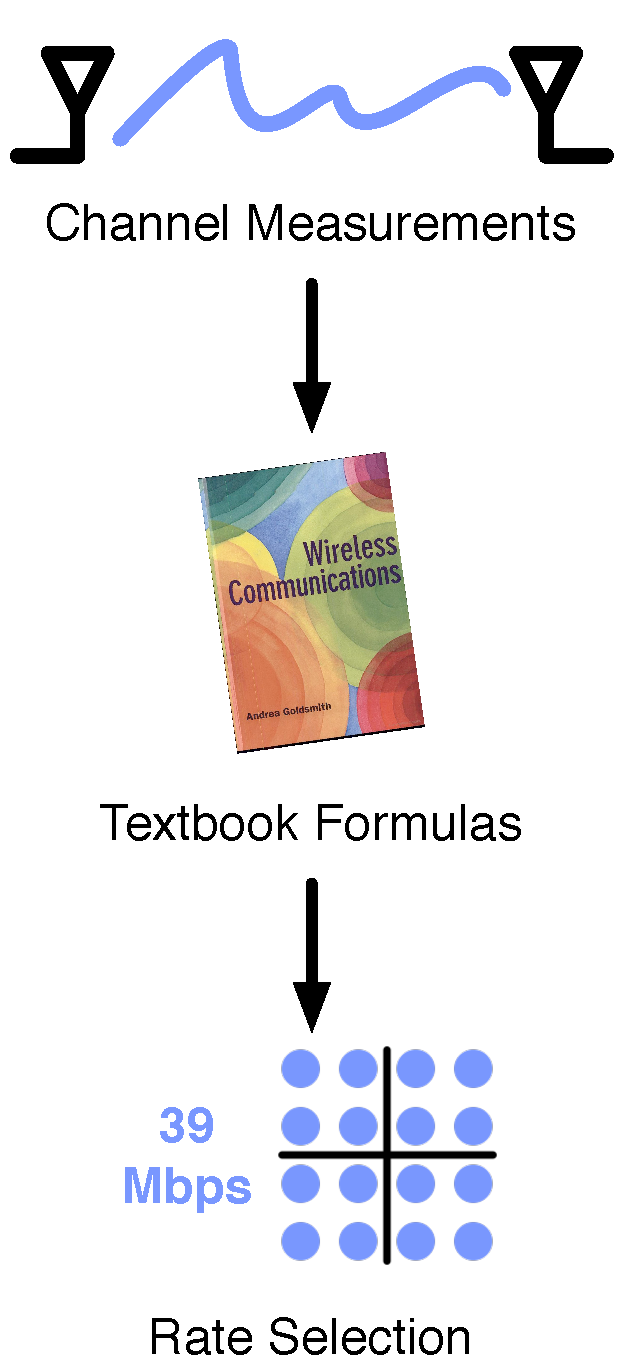
\includegraphics[width=2in]{figures/rate_selection_theory}
			\hspace{0.1in}
		}
			\hspace{0.1in}
		\subfigure[The probe-based approach to rate selection used in practice][The probe-based approach to rate selection used in practice.]{
			\hspace{0.1in}
			\label{fig:rate_selection_practice}
			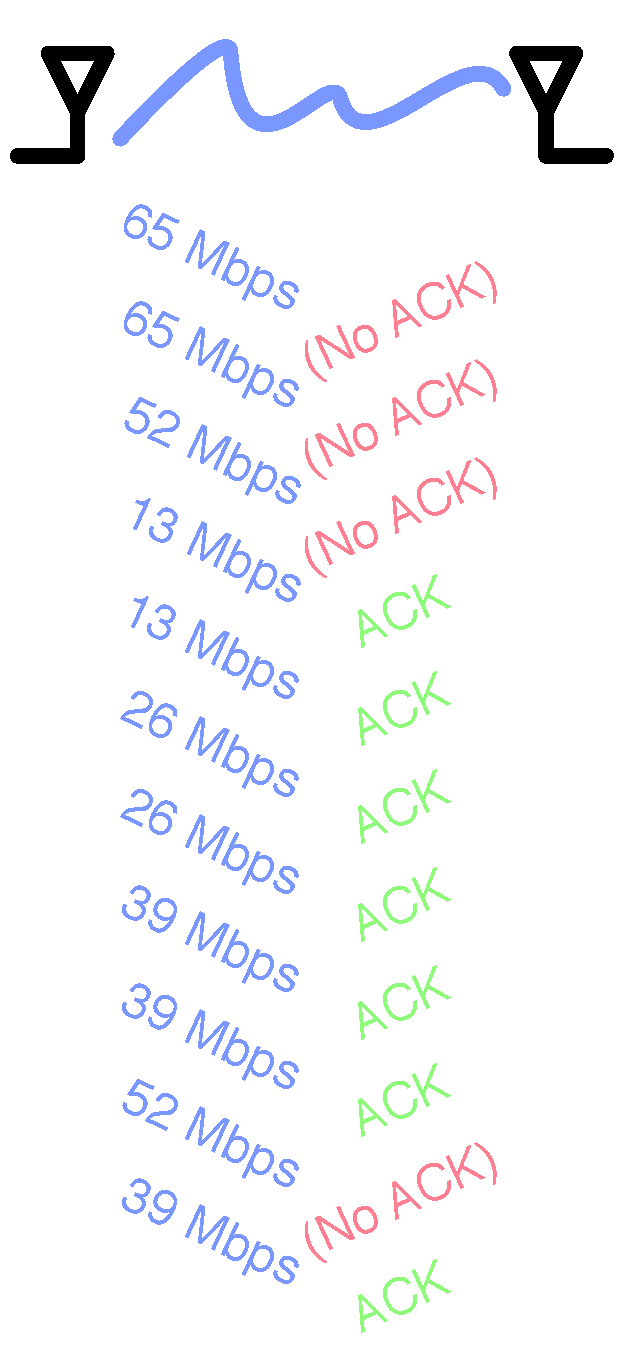
\includegraphics[width=2in]{figures/rate_selection_practice}
			\hspace{0.1in}
		}
	\caption[Approaches to rate selection]{\label{fig:rate_selection_algorithms}Approaches to rate selection.}%
\end{figure}

In practice, this approach has never worked for Wi-Fi links. The 802.11 standard defines a channel metric related to the SNR called the Receive Signal Strength Indicator, or RSSI, that captures the total amount of power in the channel and in most chipsets is indeed a direct measure of the SNR. However, Wi-Fi systems have never used RSSI as more than a coarse indicator of expected performance. There have simply been too many ways in which the observed measurements and actual performance fail to match the predictions of theory. For example, hardware estimates of RSSI can be mis-calibrated, the wireless channel can vary over packet reception, and can be corrupted by interference; all of these are known to be issues in practice~\cite{Camp_rateadapt,Judd_CHARM,Reis_interference}.

Since rate selection based on RSSI has never worked for Wi-Fi, practical systems use \define{rate adaptation} algorithms instead~\cite{Bicket_SampleRate,Minstrel,Wong_RRAA}. These algorithms, exemplified by \figref{fig:rate_selection_practice}, are guided search schemes that simply test individual rates to see how well they work. When the loss rate is too high, a lower rate is used; otherwise a higher rate is tested. This approach works well for slowly varying channels and simple links, since the best setting will soon be found.

However, remember the Wi-Fi trends we mentioned earlier: the transmit configuration of a single Wi-Fi link now includes not just rate, but additional dimensions that take into account the use of multiple antennas or channel widths, and these devices are increasingly being used while mobile. Thus algorithms to configure the rates of these links need to respond faster to match changing channels, while simultaneously choosing from among more possibilities. As a result, rate adaptation algorithms are getting less efficient as these systems change.

Thus far, I have described the challenges inherent to choosing an efficient rate to send data on a wireless link. On its own, this is a hard problem, but in addition, I note that rate is only one of many parameters to optimize for a Wi-Fi link. For instance, a transmitter may want to trim excess transmit power to both save energy and reduce interference at nearby receivers. Or a sender might improve a link by selecting a different subset of its transmit antennas, or by applying beamforming techniques to better match the signal to the radio channel. Finally, note that these parameters are not generally independent---changing any one of them can affect the best operating point for another. For instance, switching the operating frequency (of which there are often 10 to 20 options) can dramatically change the RF channel, and this in turn can affect which transmit antennas provide the best link, and how the transmitted signal should be shaped for maximum performance. All of these factors contribute to determining the best way to configure a link.

In practice, the solution taken by hardware/driver manufacturers today is to simply ignore most of these dimensions. For instance, only Intel's \program{iwlwifi} driver, out of all the 802.11n drivers in the Linux kernel driver, adapts the transmit antenna set in an online manner. Similarly, few access points and no clients adjust transmit power for ongoing links, instead opting to transmit at the maximum power and guarantee the best link. The solutions work well enough for wireless access point networks, mostly due to the simple way in which links are used today. Still, these solutions are inefficient for a single link---and in the next section, we will see that the problem gets even more complicated when performing network-level configuration of multiple devices that operate in multiple links.

\subsection{Configuring a Network of Devices}
\label{sec:intro_network_problems}
In this section, I will illustrate how a network of devices has a significantly larger configuration space than a single link. I frame this discussion using the examples in \figref{fig:network_examples}, which represent the three key network-level configuration problems that Wi-Fi Direct networks will have to solve to build rich device-to-device applications. Depending on the problem being solved, these configuration problems can have increased complexity that is linear in the number of devices (AP selection), quadratic (Multi-hop routing), or even exponential (Spatial reuse).

\begin{figure}[tp]
	\centering
	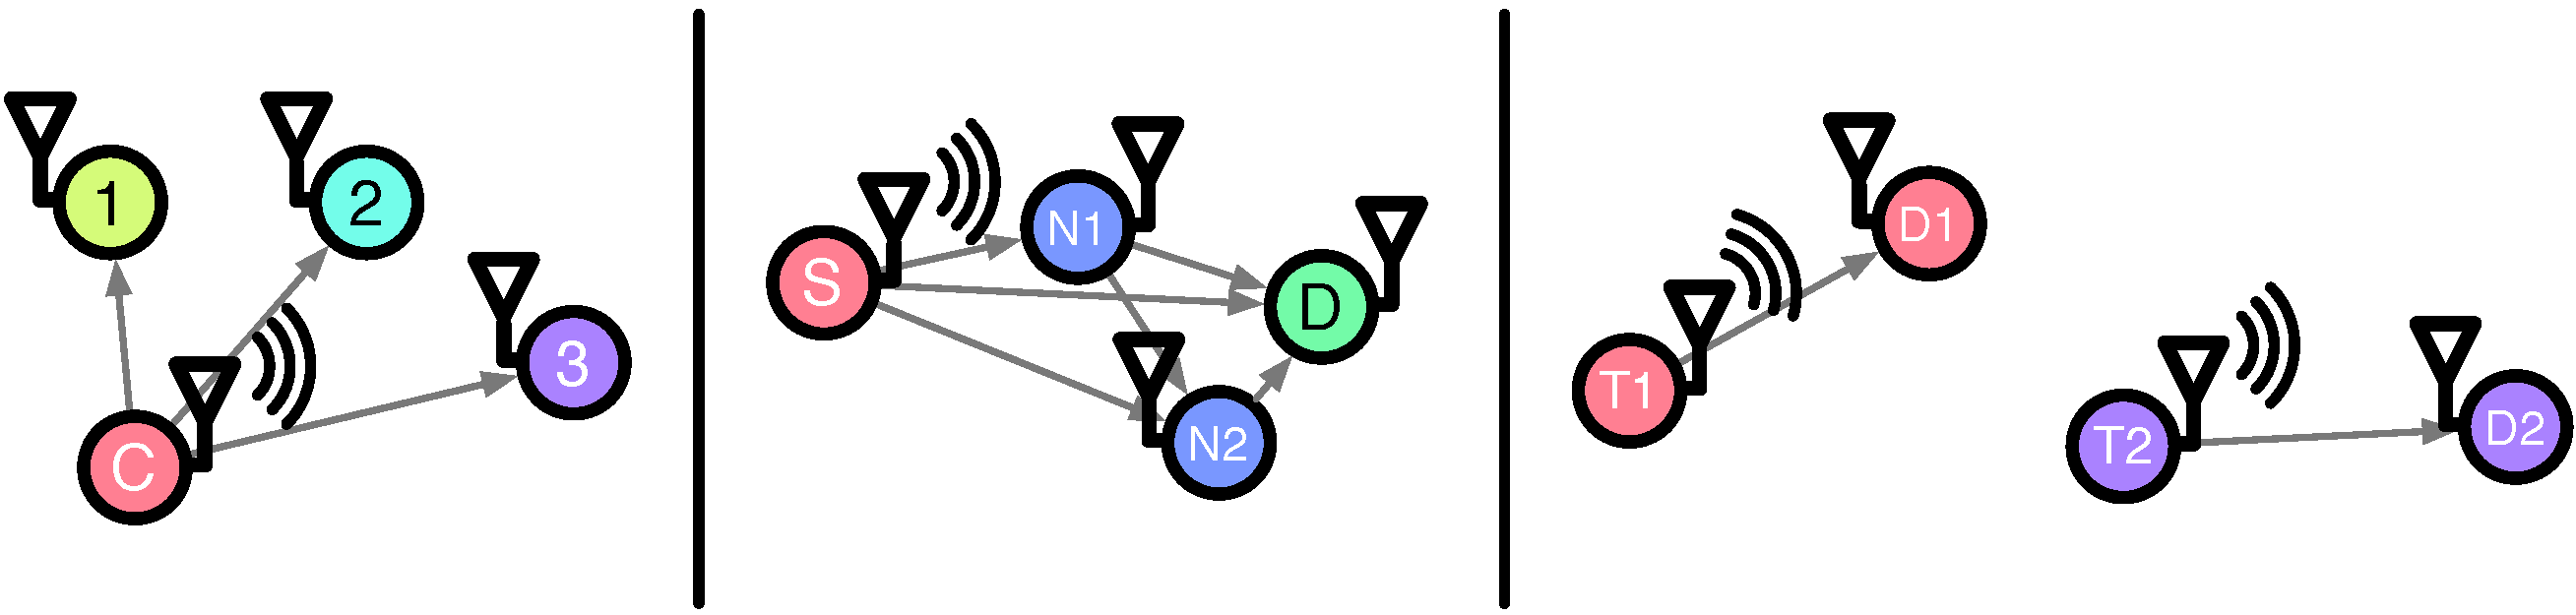
\includegraphics[width=\textwidth]{figures/network}
	\caption[The three key configuration problems in multi-device networks]{\label{fig:network_examples} The three key configuration problems in multi-device networks. \textit{Left:} access point selection. \textit{Center:} Multi-hop mesh routing. \textit{Right:} Spatial reuse. }
\end{figure}

\subsubsection{Access Point Selection}
In \figref{fig:network_examples}, on the left, the client $C$ wishes to join the network offered by the access points $AP_1$, $AP_2$, and $AP_3$. The \define{access point selection} problem is simple: the client should connect to the access point that provides the link with the best rate. But in order to choose correctly, the client must accurately evaluate the rate offered by each access point. This in turn means that the client must have a way to assess its rate to each access point rapidly, i.e., a solution to the rate selection problem described above. Testing all access points using a rate adaptation-like approach would take too long and would take airtime away from ongoing connections. In practice clients simply connect the access point with the highest SNR\@. This heuristic approach provides only an approximation to the optimal solution, and would benefit from a better way to predict performance over measured wireless channels.

\subsubsection{Multi-hop Mesh Routing}
In \figref{fig:network_examples}, in the middle, the source $S$ wishes to send data to the destination $D$, and nodes $N_1$ and $N_2$ are also present in the network. The \define{multi-hop routing} problem is to choose the best path through the network by which to deliver data from $S$ to $D$. In this case, many paths are available, such as the direct path $S\mendash D$, the one-hop paths $S\mendash N_1\mendash D$ and $S\mendash N_2\mendash D$, and finally $S\mendash N_1\mendash N_2\mendash D$. To evaluate the different paths, we need to know the rate available on each hop, which in this case would require knowing the rates of six different links. Once again, measuring the ground truth rate of each link by testing each configuration would likely take too long, and would add overhead to the network.

Practical work in this area primarily takes one of two approaches. Most of the wireless mesh research in the past decade avoided this problem by simply ignoring many of the dimensions of the configuration space. These papers not only used single antenna systems at fixed transmit powers, but also typically fixed the entire network to a single rate. The alternative approach, taken by a few recent papers, has been to collected statistics about packet delivery between all pairs of nodes for different rates, and estimate the rate from the measured SNR for links without sufficient statistics. These recent works have exclusively handled single-antenna 802.11a/b/g networks, and would likely be forced to rely on SNR-based rate predictions if the underlying links used 802.11n instead.

\subsubsection{Spatial Reuse}
The third example, shown in \figref{fig:network_examples}, is the \define{spatial reuse} problem. Here, two independent links both wish to communicate at the same time and in the same frequency, and need to share the wireless medium. If the links share the medium, for example each using half the airtime, then each gets half of the rate as if they were operating alone. In certain situations, depending on the placement of the four devices and the amount of interference between links, it may provide more total throughput for the links to send concurrently, each using all of the airtime but maybe using a slightly lower rate.

Once again, deciding which of these two possibilities is better requires the system to predict the rate on multiple different links. In this case, the rate needs to be predicted not only for each link in isolation, but also for every possible pair of configurations of the links. In this case, and unlike the prior two problems, the size of the resulting configuration space is the product of the sizes of the space of each individual link. As a result%, CMAP~\cite{Vutukuru_CMAP} and CENTAUR~\cite{Shrivastava_CENTAUR},
practical works on spatial reuse for Wi-Fi has simply fixed the entire network to a single rate during experiments.

\subsection{Summary}
In this section, I first showed that the configuration problems for a single link have grown dramatically with the switch to 802.11n technology, and then presented the three key network-level configuration problems for Wi-Fi Direct-like networks and explained why their solution space is even larger than for a single link. The main conclusion from this section is that the heuristic and adaptation-based approaches used in the simple network problems solved today will likely not scale to these bigger problems. (I will demonstrate this later in the thesis in \chapref{chap:applications}). Instead, what we need is a way to accurately and rapidly assess the quality of links for all the factors mentioned in \secref{sec:intro_single_link_problems}, and use this process to inform joint optimization problems such as those described in \secref{sec:intro_network_problems}. I present my approach to solving this problem in the next section.

%Depending on the problem being solved, these configuration problems can have increased complexity that is linear in the number of devices (AP selection), quadratic (Multi-hop routing), or even exponential (Spatial reuse). 
%Additionally, these scenarios tend to differ from the single link case in that their solutions can not be fluidly adapted while online. For instance, a transmitter on a single link could rapidly adapt its rate or antenna selection, and a poor choice will be rapidly corrected. Conversely, a client in today's wireless networks cannot switch between access point at short time scales. Thus it is especially important that these network-level decision problems are made accurately the first time.

%%%%%%%%%%%%%%%%%%%%%%%%%%%%%%%%%%
\section{Approach}
\label{sec:intro_approach}
My approach to the Wi-Fi network configuration problem is to return to the basic channel measurement-based strategy of selecting configurations for wireless networks. In particular, my hypothesis is that it is possible to use theory to connect the performance of 802.11 devices on real links to measurements of their underlying radio channels in practice. In this thesis, I will demonstrate that channel measurements readily available in 802.11n Wi-Fi devices can be used to predict packet delivery over real 802.11n links, and that these predictions are sufficiently accurate to inform decisions about wireless network device configurations.

\subsection{Better physical layer measurements}
I noted earlier that the packet-level SNR metric computed from RSSI has never been used as an accurate predictor of packet delivery for 802.11 networks, and I will present experimental data that confirms this effect in a succeeding chapter (\chapref{chap:problem}). If hardware estimates of RSSI are not sufficiently accurate, then what data source can we use instead?

The 802.11n standard released in 2009 adds a new Channel State Information (CSI)~\cite[\S7.3.1.27]{80211n} measurement facility in order to support multi-antenna (Multiple-Input-Multiple-Output, or MIMO) operation. Devices that report the CSI can provide channel measurements at the level of individual OFDM subcarriers and individual spatial paths. These measurements form a much richer set of information about the RF channel than does the RSSI.

To compare the CSI with SNR, consider an 802.11n link with $M$ antennas at the transmitter and $N$ at the receiver. Today's receivers measure $N$ RSSI values, each corresponding to the total power measured at one receive antenna. In contrast, the CSI contains $M$$\times$N$\times$$S$ values, where $S$ is the number of subcarriers measured. This results in a factor of $MS$ more channel measurements when measuring CSI as opposed to SNR\@. In 802.11, the CSI can measure from 1 to 4 antennas, and from 16 to 114 subcarriers. The CSI thus includes between 16$\times$ and $456\times$ as many measurements as the RSSI\@.

%\item Second, the quality of Wi-Fi hardware has improved dramatically. Manufacturers typically calibrate chipsets across a wide range of conditions, including temperature and transmit power level, in order to meet regulatory requirements, to meet standardized tolerances, and to maximize performance. The modern use of OFDM and MIMO techniques additionally enables channel estimates that are less susceptible to interference than spread-spectrum modulation (because of lower correlation), and can be taken more rapidly.

\subsection{A practical Effective SNR model for 802.11n}
The CSI gives fine-grained channel measurements that capture the low-level details of the physical RF channel, but this does not on its own give an accurate predictor of packet delivery. However, there is a recent body of theoretical work on measuring and predicting the error performance of wireless channels that are faded, use OFDM, or use MIMO\@. Chief among these is the seminal 1998 paper by Nanda and Rege on the concept of \define{Effective $E_b/N_0$}~\cite{Nanda_EffectiveSNR},\footnote{In electrical engineering literature, $E_b$ denotes the energy of a bit and $N_0$ denotes the noise floor, so $E_b/N_0$ is the signal-to-noise ratio of a single bit. In the context of 802.11, in which SNR is derived from RSSI, we use a slightly different definition of SNR that is not normalized by the number of bits.} which forms the theoretical basis of my model for 802.11n MIMO-OFDM channels. In this thesis, I build a practical Effective SNR-based model that uses CSI measurements from commodity 802.11n devices and makes accurate predictions about 802.11n packet delivery.

I give a detailed description of the Effective SNR concept and how I model it in a practical system in a subsequent chapter (\chapref{chap:model}). Briefly, the goal of the Effective SNR is to to give a channel quality metric that reflects the \emph{actual error rate of the link} taking into sub-channel effects like fading. The Effective SNR of a faded channel is defined as the SNR in an equivalent constant-SNR channel that would yield the same error performance. Another way to think about this is that the SNR reports the \emph{total power} received, whereas the Effective SNR reports the amount of \emph{useful power} received. As I will show in this thesis, because Effective SNR accurately reflects packet delivery it can be used to inform a wide variety of configuration decisions about 802.11n systems.

\begin{figure}[t]
	\centering
	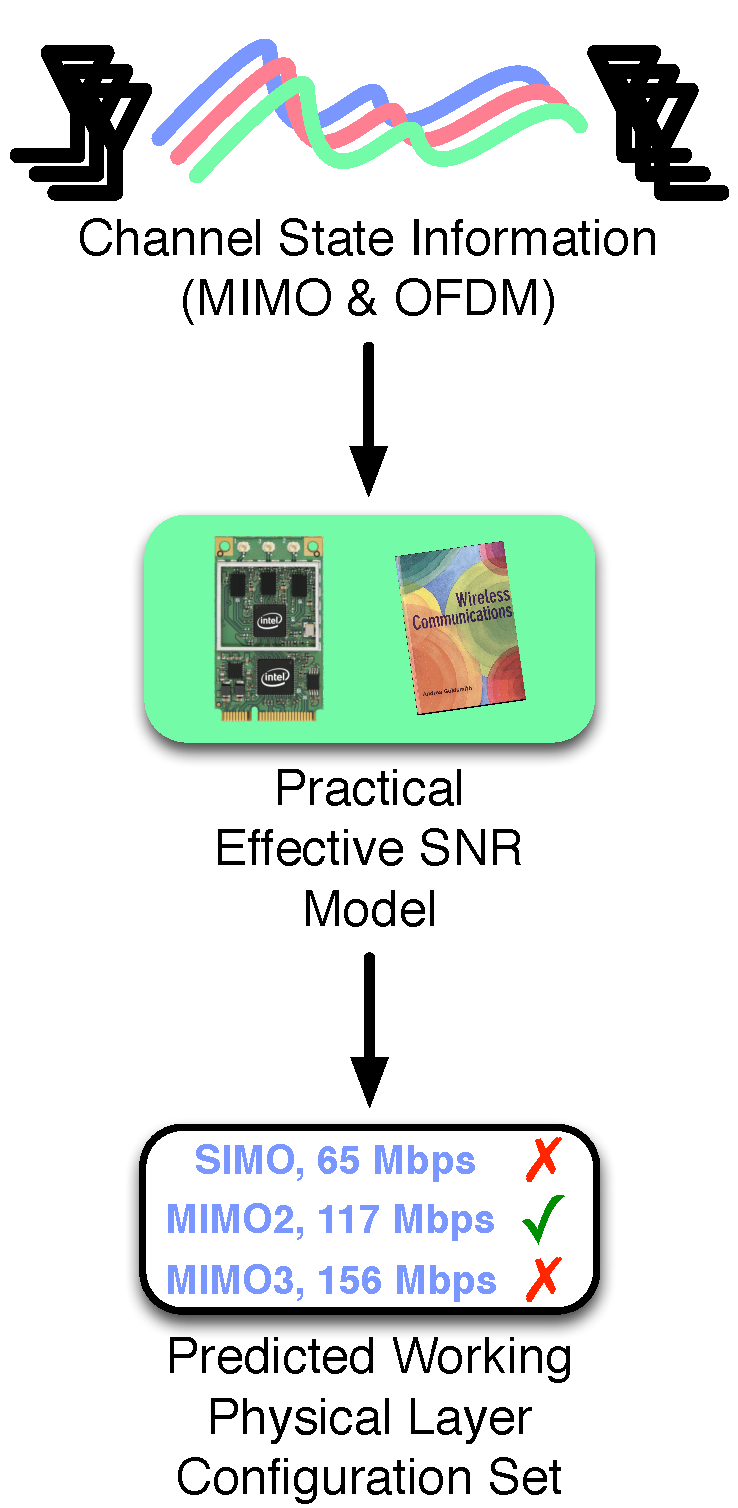
\includegraphics[width=2.2in]{figures/selection_esnr}
	\caption[Effective SNR-based approach to making application decisions]{\label{fig:selection_esnr}An Effective SNR-based approach to making application decisions in 802.11n networks.}
\end{figure}

\subsection{Approach overview}
I present the basic outline of my Effective SNR-based approach to informing configuration of 802.11n systems in \figref{fig:selection_esnr}. This approach is closely related to the ``theoretical approach'' presented in \figref{fig:rate_selection_theory}, with a few differences.

As a first step, a client will measure the CSI for an 802.11n wireless link to capture the fine-grained channels details at the level of frequency-selective fading (to understand performance under OFDM) and independent spatial paths (to understand performance when using MIMO). Second, the measured CSI will be used as input to my practical Effective SNR-based model for 802.11n packet delivery. This model incorporates textbook algorithms, ideas from communications theory, as well as some implementation-specific details to handle a wide variety of channels, hardware devices, and applications. Finally, the output of the model is a predicted \emph{set of working physical layer configurations}. For each physical layer configuration in the application space---which can span the choice of modulation, coding scheme, transmit or receive antenna set, and more---the model predicts whether that configuration is likely to deliver packets reliably. The application can then choose among the working configurations in a way that optimizes its objective function.

Throughout this thesis, I describe the components of this approach in detail. The organization of this thesis is presented below in \secref{sec:intro_organization}.

%In my thesis, I take advantage of these three points to build a practical system to return to the ``traditional'' algorithm and predict wireless error performance from channel measurements. Rather than the ``try-it-and-see'' adaptation algorithms in use today, my model enables measurement-based selection of operating points for a wide range of transmitter and receiver parameters over a large application space.

%The opportunity to make progress has arisen for two reasons. First, 802.11n devices measure the channel at the level of individual OFDM subcarriers and individual spatial paths to support 802.11n MIMO (multi-antenna) operation. They report this information in a standard Channel State Information (CSI) format~\cite[\S7.3.1.27]{80211n}. This provides a much richer source of information than SNR\@. Note that this CSI naturally applies to 802.11a/g rates because they are a subset of 802.11n rates. Second, modern NICs use OFDM, which gives channel estimates that are less susceptible to interference than spread spectrum (because of lower correlation), and are calibrated. Both factors lead to more meaningful measurements than in the past.


%\subsubsection{Better Channel Measurements}
%The chief problems with using channel measurements available in commodity Wi-Fi devices is that they only describe the SNR, a measure of total power in the channel. Even if they didn't suffer from the hardware artifacts described above, this information would insufficiently describe the wireless channel, because bits are no longer spread across the entire band as in 802.11b modes, but instead are sent independently on different frequencies (called subcarriers) with orthogonal frequency division multiplexing (OFDM), and on different spatial paths with 802.11n multi-antenna techniques.
%
%As part of my thesis, I built a tool (described in \secref{sec:tool}) to measure the channel in a fine-grained manner that accurately reflects the underlying radio channel. In particular, this tool can measure the 802.11n Channel State Information (CSI)~\cite[\S7.3.1.27]{80211n} for each received 802.11n packet. The CSI measures not just the SNR of the entire channel, but instead the channel response at the level of individual subcarriers and spatial paths. For comparison, for an 802.11n link with the antennas each at the transmitter and receiver, today's receivers measure three SNR values each corresponding to the total power measured at a receive antenna. In contrast, the CSI contains 3$\times$3$\times$$S$ values, where $S$ is the number of subcarriers measured. Since 802.11n links use either 56 or 114 subcarriers, $S$ could be as high as 56; in practice, our tool can only measure a subset of 30 of them. Still, this results in 270 channel measurements using the CSI, compared to only 3 with the traditional SNR\@.
%My tool uses a commercially-available Intel Wi-Fi device that supports 802.11n. I modified the open-source Linux drivers, and---in conjunction with Intel Research---the firmware for these devices to enable debug modes with 
%\subsubsection{Effective SNR}


%%%%%%%%%%%%%%%%%%%%%%%%%%%%%%%%%%
\section{Contributions}
\label{sec:intro_contributions}

The contributions of this thesis are threefold:
\begin{itemize}
\item First, I develop a model that uses the 802.11n CSI to predict the error performance of different transmitter configurations on the wireless channel. This model is flexible to support a wide variety of transmitter and receiver device capabilities, device implementations, and applications. I also detail how to use this model in a system that can solve a large number and variety of configuration problems similar to those described in \secref{sec:intro_problem}.
\item Second, I present an implementation of this system using a commodity 802.11n wireless device that demonstrates its feasibility in practice and handles the practical considerations of operation over real links using real, non-ideal hardware. This includes a detailed experimental evaluation of my system that shows that this model accurately predicts packet delivery over real 802.11n wireless links in practice.
\item Third, I evaluate this system in the context of a wide variety of 802.11n applications, and quantify the application performance gains when using my Effective SNR metric over versions that use the RSSI-based SNR channel measurements available today.
\item Finally, as part of my thesis I have produced an 802.11n research platform based on open-source Linux kernel drivers, open-source application code, and commodity Intel 802.11n devices using closed-source firmware that I customized.
%that uses commodity 802.11n wireless devices to measure the 802.11n CSI for the wireless channel, and use this tool to apply my model to real measured 802.11n channels.
I have released this tool publicly, and at the time of writing it is in use at 19 universities, research labs, and corporations.
\end{itemize}

%%%%%%%%%%%%%%%%%%%%%%%%%%%%%%%%%%
\section{Organization of this Thesis}
\label{sec:intro_organization}
This thesis is organized as follows. In \chapref{chap:background}, I provide background information on wireless signals and systems in general, and the IEEE 802.11 standards in particular. \chapref{chap:problem} introduces the problem with using channel measurements to predict wireless link performance in today's hardware and using today's techniques, and introduces my Effective SNR-based approach to solving it. In \chapref{chap:model}, I develop my Effective SNR model for 802.11n link performance, and demonstrate its ability to handle a wide range of transmitter and receiver configurations as well as wireless applications. I then describe my measurement tool, experimental apparatus, and basic measurements in \chapref{chap:tool}, and then use these measurements to evaluate the ability of my model to predict error performance over a single link in \chapref{chap:delivery}. Next, I conduct a detailed study of the model in the context of rate selection for 802.11n in \chapref{chap:rate}, and then present brief results for a variety of other applications in \chapref{chap:applications}. I place this thesis in the context of related work in \chapref{chap:related}. Finally, I present a brief discussion of the next steps for this work along with concluding thoughts in \chapref{chap:conclusion}.

%%%%%%%%%%%%%%%%%%%%%%%%%%%%%%%%%%
\ifx\mainfile\undefined
%
% ==========   Bibliography   ==========
%
%\nocite{*}   % include everything in the uwthesis.bib file
\bibliographystyle{plain}
\bibliography{dhalperi_thesis}

\end{document}
\fi

\ifx\mainfile\undefined
%  ========================================================================
%  Copyright (c) 2006-2011 The University of Washington
%
%  Licensed under the Apache License, Version 2.0 (the "License");
%  you may not use this file except in compliance with the License.
%  You may obtain a copy of the License at
%
%      http://www.apache.org/licenses/LICENSE-2.0
%
%  Unless required by applicable law or agreed to in writing, software
%  distributed under the License is distributed on an "AS IS" BASIS,
%  WITHOUT WARRANTIES OR CONDITIONS OF ANY KIND, either express or implied.
%  See the License for the specific language governing permissions and
%  limitations under the License.
%  ========================================================================
%
 
\documentclass [11pt, twoside] {uwthesis}

\usepackage{color}
\usepackage{url}
\usepackage{amsmath}
\usepackage{amsfonts}
\usepackage[bookmarks,
	hidelinks,
	plainpages=false,
	pdfpagelabels,
	pagebackref=true,
            ]{hyperref}
\renewcommand*{\backref}[1]{}% for backref < 1.33 necessary
\renewcommand*{\backrefalt}[4]{%
  \ifcase #1 %
    (No citations.)%
  \or
    (Cited on page #2.)%
  \else
    (Cited on pages #2.)%
  \fi
}

\newcommand{\biburl}[1]{{\tt<}\url{#1}{\tt>}}

\hypersetup{%
pdfauthor = {Daniel Chaim Halperin},
pdftitle = {Simplifying the Configuration of 802.11 Wireless Networks with Effective SNR},
pdfsubject = {Ph.D. Dissertation},
pdfkeywords = {},
pdfcreator = {University of Washington, Computer Science and Engineering},
pdfproducer = {},
bookmarksopen = {true},
pdfpagelayout = {TwoColumnRight},
}

\usepackage{footnotebackref}
%%%%%%%%%%%%%%%%%%%%%%%%%%%%%%%%%%%%%%%%%%%%%%%%%%%%%%
%%%        Formatting sections                     %%%
%%%%%%%%%%%%%%%%%%%%%%%%%%%%%%%%%%%%%%%%%%%%%%%%%%%%%%
\newcommand{\algref}[1]{Algorithm~\ref{#1}}
\newcommand{\chapref}[1]{Chapter~\ref{#1}}
\renewcommand{\eqref}[1]{Equation~\ref{#1}}
\newcommand{\figref}[1]{Figure~\ref{#1}}
\newcommand{\secref}[1]{\S\ref{#1}}
\newcommand{\tabref}[1]{Table~\ref{#1}}
\newcommand{\heading}[1]{\vspace{4pt}\noindent\textbf{#1}}
\newcommand{\topheading}[1]{\noindent\textbf{#1}}
\newcommand{\noheading}[0]{\vspace{4pt}\noindent}

%%%%%%%%%%%%%%%%%%%%%%%%%%%%%%%%%%%%%%%%%%%%%%%%%%%%%%
%%%        XXX and other warnings                  %%%
%%%%%%%%%%%%%%%%%%%%%%%%%%%%%%%%%%%%%%%%%%%%%%%%%%%%%%
\newcommand{\xxx}[1]{\textit{\color{red}XXX #1}}

%%%%%%%%%%%%%%%%%%%%%%%%%%%%%%%%%%%%%%%%%%%%%%%%%%%%%%
%%%        Units                                   %%%
%%%%%%%%%%%%%%%%%%%%%%%%%%%%%%%%%%%%%%%%%%%%%%%%%%%%%%
\usepackage{xspace}
\newcommand{\unitsep}{\texorpdfstring{\,}{ }}
\def\unit#1{% from: http://www.tex.ac.uk/cgi-bin/texfaq2html?label=csname "Defining a macro from an argument"
  \expandafter\def\csname #1\endcsname{\unitsep\text{#1}\xspace}%
}
\def\varunit#1#2{% from: http://www.tex.ac.uk/cgi-bin/texfaq2html?label=csname "Defining a macro from an argument"
  \expandafter\def\csname #1\endcsname{\unitsep\text{#2}\xspace}%
}
\unit{GHz}
\unit{MHz}
\unit{kHz}
\unit{Gbps}
\unit{Mbps}
\unit{KB}
\unit{dB}
\unit{dBi}
\unit{dBm}
\unit{W}
\unit{mW}
\varunit{uW}{$\mu$W}
\unit{ms}
\varunit{us}{$\mu$s}
\unit{h}
\unit{m}
\unit{s}
\unit{km}
\unit{cm}
\unit{mm}
\varunit{mmsq}{mm$^\text{2}$}
\varunit{insq}{in$^\text{2}$}
\newcommand{\degree}{\ensuremath{^\circ}\xspace}
\newcommand{\degrees}{\degree}
%%%%%%%%%%%%%%%%%%%%%%%%%%%%%%%%%%%%%%%%%%%%%%%%%%%%%%%%%%%%%%%%%%%%%%%%%%%%%%%%%%%%%%
% Euler for math | Palatino for rm | Helvetica for ss | Courier for tt
%
% From: http://www.tug.org/mactex/fonts/LaTeX_Preamble-Font_Choices.html
%%%%%%%%%%%%%%%%%%%%%%%%%%%%%%%%%%%%%%%%%%%%%%%%%%%%%%%%%%%%%%%%%%%%%%%%%%%%%%%%%%%%%%
\renewcommand{\rmdefault}{ppl} % rm
\usepackage[scaled]{helvet} % ss
\usepackage{courier} % tt
\usepackage{eulervm} % a better implementation of the euler package (not in gwTeX)
\normalfont
\usepackage[T1]{fontenc}
%%%%%%%%%%%%%%%%%%%%%%%%%%%%%%%%%%%%%%%%%%%%%%%%%%%%%%%%%%%%%%%%%%%%%%%%%%%%%%%%%%%%%%

%%%%%%%%%%%%%%%%%%%%%%%%%%%%%%%%%%%%%%%%%%%%%%%%%%%%%%
%%%        Figures                                 %%%
%%%%%%%%%%%%%%%%%%%%%%%%%%%%%%%%%%%%%%%%%%%%%%%%%%%%%%
\usepackage{graphicx}
% Caption package both lets you set the spacing between figure and caption
% and also makes the \figref{} point to the right place.
\usepackage[font=bf,aboveskip=6pt,belowskip=-4mm]{caption}
% Allow subfigures, make them bold
\usepackage[bf,BF,small]{subfigure}
% List of figures
\setcounter{lofdepth}{2}  % Print the chapter and sections to the lot

%%%%%%%%%%%%%%%%%%%%%%%%%%%%%%%%%%%%%%%%%%%%%%%%%%%%%%
%%%        Lists with reduced spacing              %%%
%%%%%%%%%%%%%%%%%%%%%%%%%%%%%%%%%%%%%%%%%%%%%%%%%%%%%%
\usepackage{enumitem}

%%%%%%%%%%%%%%%%%%%%%%%%%%%%%%%%%%%%%%%%%%%%%%%%%%%%%%
%%%        Fancy tables                            %%%
%%%%%%%%%%%%%%%%%%%%%%%%%%%%%%%%%%%%%%%%%%%%%%%%%%%%%%
\usepackage{tabulary}
\usepackage{booktabs}

%%%%%%%%%%%%%%%%%%%%%%%%%%%%%%%%%%%%%%%%%%%%%%%%%%%%%%
%%%        Formatting techniques/tools/etc.        %%%
%%%%%%%%%%%%%%%%%%%%%%%%%%%%%%%%%%%%%%%%%%%%%%%%%%%%%%
\newcommand{\term}[1]{\texttt{#1}}

\begin{document}
 
\textpages
\setcounter{chapter}{1} % Set to n-1!
\fi
%%%%%%%%%%%%%%%%%%%%%%%%%%%%%%%%%%

\cleardoublepage
\chapter{Background}
\label{chap:background}

In this chapter, I establish the fundamentals of wireless communication and the IEEE 802.11 standards to the extent needed to understand my thesis.

\section{Digital Communication Principles}
Electromagnetic (EM) communications, which send data using \define{electromagnetic signals}, form the basis of the technologies I will discuss in this thesis. One key aspect of each wireless technology is which part of the electromagnetic spectrum it uses, characterized by its \define{carrier frequency or center frequency}, denoted $f$. A fundamental property of radio waves is that the frequency of a wave determines its \define{wavelength} $\lambda$ according to the relationship $c=f\lambda$, where $c$ is the speed of light. IEEE~802.11 networks typically use EM signals with a carrier frequency in the range of 2.4\GHz and 5\GHz and corresponding wavelengths of about 12\cm and 6\cm.

Data transmission using EM signals works by \define{modulating} a pure sine wave with frequency $f$, i.e.\ by transforming the sine wave to reflect the underlying data. The simplest modulation scheme might be to turn the sine wave on or off depending on whether the bit to be transmitted is a 1 or a 0. The rate at which the transmitter varies the signal---in this example, the rate the sine wave is turned on or off---is called the \define{symbol rate}, and determines the \emph{bandwidth} of the channel $B$ measured in Hertz (Hz).

The \emph{amplitude} of the sine wave, e.g. how much the peak varies from the zero (usually measured in volts (V)), determines the \define{power} of the signal. These two quantities are related by a quadratic relationship: doubling the amplitude of a signal results in a quadrupling of the signal power.

In a \define{link}, that is a sender communicating data to a receiver, the sender generates a signal with \define{transmit (signal) power} level $T$ that propagates through the \define{channel} connecting the two. The channel could be a \define{wire} or it could be the free-space \define{radio frequency (RF)} environment in which signals propagate from the transmitter's antenna to the receiver's antenna over the air.

\subsection{The Wired Channel}
To simplify the discussion, I will start with the case of a wired channel. The transmitted signal propagates down the wire to the receiver and then is received with \define{receive (signal) power} $S$. While propagating through the wire, the signal gets slightly weaker as a small amount of energy is absorbed. The net effect of this absorption is called \define{attenuation}, denoted $\alpha$, and is defined mathematically as the multiplicative decrease in power induced by the channel:
\begin{equation}
	\label{eq:attenuation}
	\alpha = \frac{T}{S}.
\end{equation}
In addition to attenuation, the wired channel also induces a \define{phase shift} as the electromagnetic signal propagates. The value of this phase shift, denoted $\theta$, depends on factors including the length of the wire and the frequency of the signal, and is generally considered to be an unknown, uniformly random quantity between $0$ and $2\pi$.

\begin{table}
\centering
\begin{tabular}{cll}
\toprule%
Variable & Meaning & Units\\
\midrule%
$f$ & Frequency & Hz \\
$\lambda$ & Wavelength & m \\
$B$ & Bandwidth & Hz \\
$T$ & Transmit signal power & dBm (decibels relative to 1 milliwatt) \\
$S$ & Receive signal power & dBm \\
$\alpha$ & Attenuation & dB (decibels, unitless) \\
$\theta$ & Phase & radians \\
$N$ & Noise power & dBm \\
$K$ & Temperature & kelvins \\
$\rho$ & Signal-to-noise ratio (SNR) & dB \\
$R$ & Shannon Capacity & bits \\
$d$ & Distance & m \\
$n$ & Path loss exponent & unitless \\
$I$ & Interference power & dBm \\
$\rho_I$ & SINR & dB \\
$M$ & Number of transmit antennas & (antennas) \\
$N$ & Number of receive antennas & (antennas)\\
\bottomrule
\end{tabular}
\caption[Table of notation used in this chapter]{\label{tab:bg_notation}Table of notation used in this chapter.}
\end{table}

The signal measured by the receiver is also corrupted by broad-spectrum electromagnetic noise. This corruption is sometimes called \define{Johnson-Nyquist noise} after its identification in 1927 by Johnson~\cite{Johnson_noise} and explanation in 1928 by Nyquist~\cite{Nyquist_noise}, but it is more commonly known as \define{thermal noise}. Thermal noise can be modeled as a complex Gaussian with average \define{noise power} $N$ (in Watts) equal to
\begin{equation}
\label{eq:noise}
N = kKB,
\end{equation}
where $k\approx1.38\times10^{-23}$ (in Joules/kelvin) is Boltzmann's constant, $K$ is the temperature (in kelvins), and $B$ is the bandwidth. This is called additive, white Gaussian noise (AWGN).
%For a device at room temperature ($\approx$ 293\K), we can compute $N$ in dBm using the approximation
%\begin{equation}
%N \text{ (dBm)} = -174 + 10\log_{10}(B).
%\end{equation}

In the context of 802.11, we typically measure power-related quantities on a logarithmic scale to capture the wide range of possible values. Power levels such as the quantities $T$, $S$, and $N$ are usually measured in decibels relative to 1~milliwatt, or dBm, and typically take on values like $T=20\dBm$ (100\mW) and $S=-80\dBm$ ($10^{-8}$\mW or 10\pW). To calculate $N$, we can use \eqref{eq:noise}: Wi-Fi links typically use bandwidths $B$ of 20\MHz or 40\MHz, which correspond to thermal noise levels of $-$101\dBm and $-$98\dBm at room temperature. In practice, the total noise is assumed to be thermal noise plus a 5\dB--15\dB \define{noise figure}, which is a quantity that estimates additional error added by imperfect analog hardware used in receiver processing. The total noise for a 20\MHz Wi-Fi channel might then be in the range of $-91$\dBm.

Now that we have defined the signal and noise powers, we can discuss the limits of the communication channel. In their seminal works, Ralph Hartley~\cite{Hartley_law} and Claude Shannon~\cite{Shannon_coding,Shannon_capacity} proved that the \define{capacity} of a channel---i.e., the maximum data rate $R$ at which the transmitter and receiver can communicate---is determined by the channel's bandwidth and its \define{signal-to-noise ratio (SNR)}. The SNR, denoted by $\rho$, is a unitless quantity typically measured in decibels and calculated as
\begin{equation}
\rho = \frac{S}{N}.
\end{equation}
For the example signal power of $-80\dBm$ and noise power of $-91\dBm$, this corresponds to an SNR of $11\dB$.


The Shannon-Hartley Theorem~\cite{Shannon_capacity} establishes what is called the \define{Shannon capacity} to be
\begin{equation}
\label{eq:shannon_capacity}
R = B\log_2(1+\rho).
\end{equation}
\figref{fig:shannon} shows this relationship for the normalized quantity $R/B$.

\begin{figure}[tb]
\centering
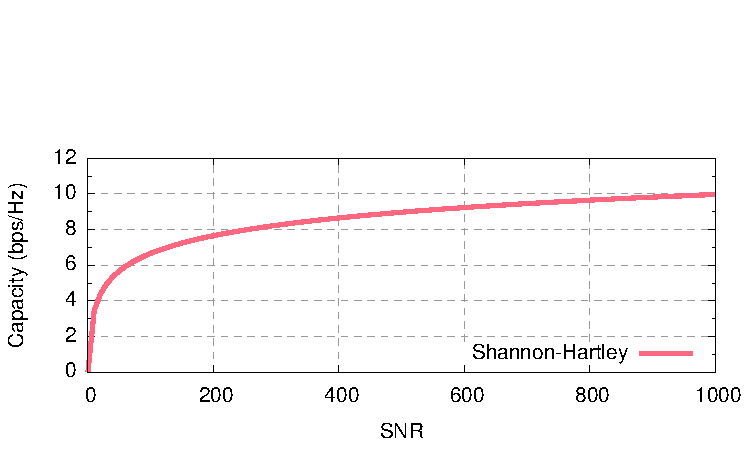
\includegraphics{calculations/shannon}\hspace{0.65in}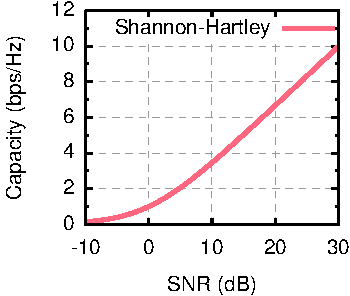
\includegraphics{calculations/shannon_log}\hspace{0.1in}
\caption[The Shannon Capacity of a communications channel with Gaussian noise]{\label{fig:shannon}The Shannon Capacity of a communications channel with Gaussian noise, presented in both linear and logarithmic (dB) scales.}
\end{figure}

The Shannon-Hartley Theorem determines a bound on the maximum rate achievable as a function of the bandwidth and signal strength. However, it does not give a practical scheme that realizes this bound, and instead systems like 802.11 use many different modulations that achieve different points along the $y$-axis, and choose among these in practice depending on the underlying channel conditions.

Note that for real links, the values of $S$ and $N$ are not known a priori. Instead, transmitters choose an encoding, and the receiver will be able to decode it successfully if the choice falls below the curve for the SNR experienced. The general problem of choosing the modulation to use, as well as the selection of other physical layer parameters, is the focus of my thesis. I describe this problem in more detail in the next chapter.

The binary modulation system I discussed above is a scheme called On-Off Keying~(OOK\@). Each symbol conveys 1 bit, and since the symbol rate is directly tied to the bandwidth used by a scheme, OOK can deliver at most 1 bps/Hz. A generalized form of OOK is Amplitude Shift Keying~(ASK\@), which can send more bits per symbol using multiple power levels. $m$-ASK, i.e., ASK with $m$ power levels per symbol, can deliver up to $\log_2(m)$ bits per symbol and thus can achieve a higher capacity.

\begin{figure}[t]
\centering
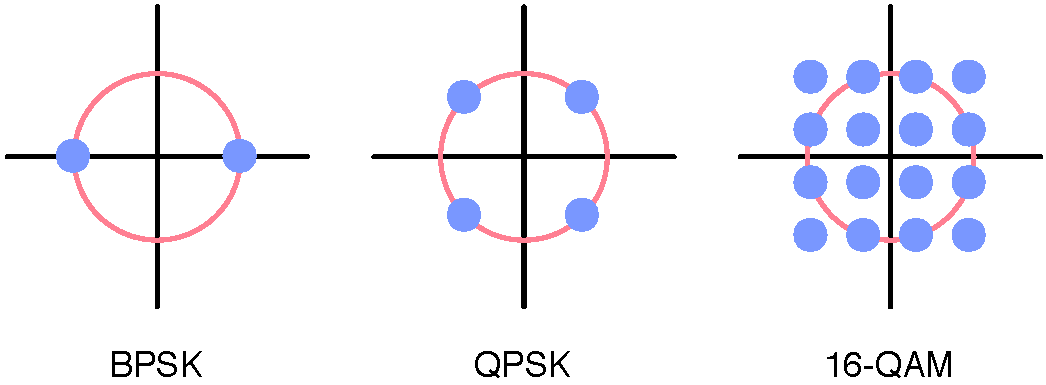
\includegraphics[width=0.9\textwidth]{figures/constellations_radius}
\caption[Constellation diagrams for the BPSK, QPSK, and 16-QAM modulations]{\label{fig:constellations}Constellation diagrams for the BPSK, QPSK, and 16-QAM modulations. These constellations are normalized such that each modulation has equal average transmit power, indicated by the red circle.}
\end{figure}

As mentioned above, electromagnetic signals actually have both an amplitude and a phase. Amplitude modulation varies one of these parameters, and a complementary scheme called Phase-Shift Keying~(PSK) keeps the amplitude constant but varies the phase. A third scheme known as Quadrature Amplitude Modulation~(QAM) varies both parameters simultaneously and results in a more efficient system when sending more than 2 bits per symbol. Noting that the polar coordinates given by amplitude and phase can equivalently be thought of as a complex number, $m$-QAM can be equivalently thought of as $\sqrt{m}$-ASK in both the real and complex dimensions simultaneously. \figref{fig:constellations} shows the two-dimensional \define{constellations} that result from picturing the symbols sent in BPSK (i.e.\ 2-PSK), QPSK (i.e.\ 4-PSK), and 16-QAM modulation schemes.

There are many more modulation schemes than I have presented here, but PSK and QAM are the modulations applicable to 802.11.
%Currently, Wi-Fi devices transmit data using 2-PSK (called Binary PSK, or BPSK), 4-PSK (called Quadrature PSK\@, or QPSK\@), 16-QAM\@, or 64-QAM\@.
64-QAM is the highest modulation currently used by Wi-Fi devices, though the future IEEE 802.11ac amendment~\cite{80211ac} will add 256-QAM to this set.

Recall that the signal will be corrupted by noise when measured at the receiver. Under the standard AWGN model, we model this corruption as shifting the received symbol by a random complex vector whose length depends on the noise power. We see in \figref{fig:constellations} that the different modulations have different constellation densities: the symbols of 16-QAM are clustered more closely than the symbols of QPSK or BPSK. This means that higher constellations which encode more bits per symbol are more vulnerable to noise. At low SNR, the receiver cannot easily distinguish between many symbols, so slower modulations with fewer constellation points should be used. At high SNR, the receiver can distinguish between more symbols and thus can use a denser constellation.

\begin{figure}[t]
\centering
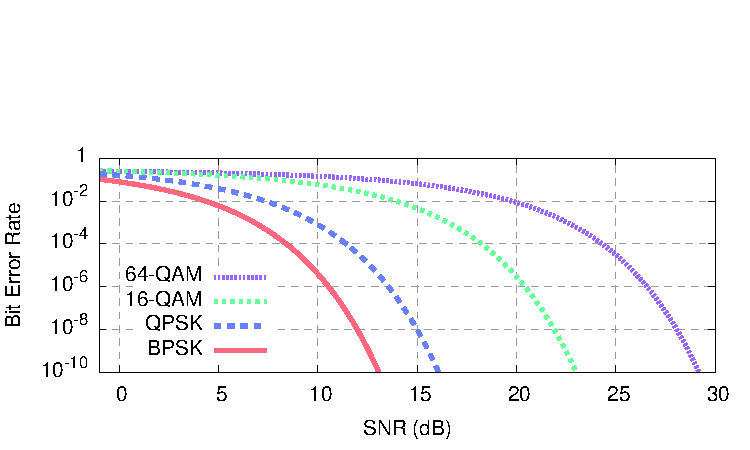
\includegraphics{calculations/snr_ber}
\caption[BER vs SNR for the four 802.11n modulation schemes]{\label{fig:mod_ber_snr}The relationship between bit error rate and SNR for the four 802.11 modulation schemes.}
\end{figure}

\begin{figure}[t]
\centering
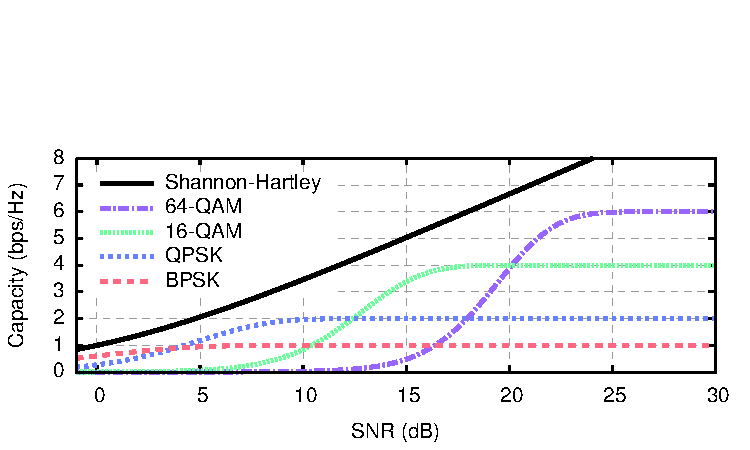
\includegraphics{calculations/snr_bits}
\caption[Capacity vs SNR for 802.11n modulation and coding schemes]{\label{fig:mod_bits_snr}The relationship between SNR and capacity for standard modulation schemes and idealized codes.}
\end{figure}

This property of the performance of different modulation schemes is closely related to the Shannon Capacity. \figref{fig:mod_ber_snr} illustrates the magnitude of this effect for the modulations used by 802.11 using textbook formulas~\cite{Sklar} that relate the SNR to a bit error rate. We can also connect these different modulations directly to the Shannon-Hartley Capacity Theorem by examining the capacity achieved by each scheme as a function of SNR (\figref{fig:mod_bits_snr}). In this graph, I assume an idealized coding scheme that delivers the maximum data rate for a given bit error rate; the practical schemes in widespread use today are somewhat less efficient in order to admit less expensive computation.\footnote{Though beyond the scope of this thesis, a number of recent proposals for practical \define{rateless codes}~\cite{Gudipati_Strider,Perry_Spinal} nearly achieve the Shannon Capacity bound by using much denser constellations and clever coding schemes across multiple transmissions.}

\subsection{The Wireless Channel}
The previous section explained the basics of digital communications in the context of a wired link. Here, I expand to the significantly more complex case of a wireless channel.

In a wireless link, the electromagnetic signal is emitted from an antenna as a \define{radio wave} that then radiates through the \define{wireless medium}, i.e.\ the environment. The dominant source of attenuation in an wireless link is not absorption by the medium, but rather the diffusion of energy throughout the environment, of which a small fraction is captured by a receiver's antenna. This effect, called \define{path loss}, is captured by the Friis transmission equation, which yields the inverse relationship
\begin{equation}
\label{eq:friis}
	S \propto \frac{T}{d^n},
\end{equation}
where $d$ is the distance between transmitter and receiver, and $n$ is the path loss exponent. In free space, $n$ has a value of 2, reflecting the fact that the energy transmitted at a particular time is spread out over the two-dimensional surface of a sphere, an area that grows with $d^2$. (For a directional antenna, the energy is spread over a different geometric shape, e.g. a cone, but this shape will still have a two-dimensional surface area).

The path loss exponent varies in different indoor environments, but empirically tends to take on a value between 2 and 4~\cite{Sklar}. This empirical result is explained as the sum of many complex effects that result from the interaction of radio waves with objects in the environment. One such effect is \define{shadowing}, in which materials such as glass or metal prevent radio waves from passing through. I explain more additional, more complicated channel effects below.

In wireless systems, multiple devices might send at the same time and in the same frequency band; this \define{interference} causes a \define{collision} during which a receiver will measure the sum of both transmissions. There are a number of practical problems for operation during a collision, such as whether the receiver can properly lock onto the desired signal and estimate the effects of the channel on it. In general, however, we can model the reception probability by replacing the SNR with the \define{signal-to-interference-and-noise ratio (SINR)}, which treats the interfering signal of power $I$ as another source of noise:
\begin{equation}
\label{eq:sinr}
\rho_I = \frac{S}{I+N}.
\end{equation}
While interference is an important problem, many systems, including 802.11, use \define{medium access control (MAC)} protocols to ensure that at most one device transmit at a time.

Beyond path loss, the most important channel effect is the inherent \emph{multi-path} nature of indoor wireless environments. At 2.4\GHz and 5\GHz, RF signals bounce off metal and glass surfaces that are common indoors. This scattering leads to a situation in which many copies of the signal arrive at the receiver having traveled along many different paths. The net effect of this RF superposition depends on the phases of the individual signals. When these copies combine they may add constructively, giving a good overall signal, or destructively, mostly canceling the overall signal.

The phase-dependent nature of multi-path effects means that they vary over both frequency and space. For a given distance traveled $d$, the phase change is $2\pi d/\lambda$. Thus wideband channels may exhibit dramatically different received power levels for different frequencies; such channels are called \define{frequency selective}. Measurement studies of frequency-selective fading report signal variations as high as 15--20\dB~\cite{Judd_CHARM}; in \chapref{chap:problem} I will present experimental evidence confirming these effects in the environments I studied.

With regard to spatial variation, the small 12\cm and 6\cm wavelengths of Wi-Fi signals means that small changes in path lengths can alter a situation from good to bad. Statistical models tell us that multi-path fading effects are independent for locations separated by as little as half a wavelength. This means that multi-path causes rapid signal changes or fast fading as the receiver moves, or in the case of a stationary node as the surrounding environment changes.  Movement at fast speed also induces \define{Doppler effect}, which aggravates multi-path effects and makes the channel even more variable.
%This means that some unlucky frequencies in a wide channel may be wiped out while others are unaffected.

The net effect of multi-path fading is that the received wireless signal can vary significantly over time, frequency and space. This is a problem for good performance because at any given time there is a significant probability of a deep fade that will reduce the SNR of the channel below the level needed for a given communication scheme.

However, an alternative way of looking at the effects of multi-path fading is that they provide \define{diversity}. In a sufficiently rich multi-path environment, there are so many combining copies of signals that the channel observed on different, nearby frequencies can be considered to be independently faded. For this reason among others, many systems including 802.11 use a scheme called Orthogonal Frequency Division Multiplexing (OFDM). In OFDM, a wide frequency band is split into many \define{subcarriers} that each carry different modulated bits in parallel, with a higher level error-correcting code across them to take advantage of this \define{frequency diversity}.

To get fast rates while only using sending a single symbol at a time, a wideband system must have a fast symbol rate. Since OFDM sends many symbols in parallel on smaller subcarriers, an OFDM system sends each symbol for a longer period of time. Thus by turning a single fast channel into many parallel slower channels, OFDM allows more time for the channel to average out temporal fades and provides \define{time diversity}.

One more type of diversity is \emph{spatial diversity}: antennas separated by at least half a wavelength see independently-faded channels. Devices with multiple antennas can use schemes that take advantage of the spatial diversity these antennas provide. For example, a multi-antenna receiver measures multiple independent copies of each transmitted signal. Thus with clever signal processing, such a receiver can align the phases of these copies and add them together, which averages out the noise and improves overall channel performance. In a complementary manner, a multi-antenna transmitter with knowledge of the fading properties of the individual paths between pairs of antennas can steer its signal such that the multiple copies arriving at the receiver's antenna combine optimally. This process, in which the gain and phase of the signal emitted by each antenna are adjusted (with OFDM, this adjustment may be different for each subcarrier) is called \define{beamforming}.
%A different technique called \define{space-time codes} to achieve the same effect, but 

Finally, suppose that both the transmitter and receiver have multiple antennas. The foundational work by Foschini, Gans~\cite{Foschini_Gans} and Telatar~\cite{Telatar_MIMO} in the mid 1990s introduced \define{spatial multiplexing}, which uses this new spatial degree of freedom to improve capacity. Instead of sending the same data out each antenna as above, a transmitter with $M$ antennas can use its different antennas to send up to $M$ independent \define{spatial streams} of data. An $N$-antenna receiver will then measure $N$ copies of each stream, each antenna an independent linear combination of the $M$ transmitted streams. If $M \leq N$, the receiver has enough information to solve the linear system and separate the streams, thus providing an $M$-fold gain in performance. Thus spatial multiplexing, with $N$ antennas at each side, results in a modified capacity theorem:
\begin{equation}
\label{eq:mimo_capacity}
R = BN\log_2(1+\rho).
\end{equation}
Together, spatial diversity and spatial multiplexing techniques form a set of what are called MIMO (multiple-input, multiple-output) techniques.

I conclude this discussion by mentioning one last channel effect relevant to 802.11: \define{inter-symbol interference}. In multi-path environments, some spatial paths can be so long that the delayed copies of the signal substantially overlap with the next symbol and make it harder to receive. The delay between the earliest and latest copies is called the \define{delay spread} of the channel, and it can be substantial. OFDM systems that use longer symbol times are more resilient to this effect, but still repeat each symbol for a period of time called a \define{guard interval}. If the guard interval is at least as long as the delay spread, the receiver can ignore the inter-symbol interference and still receive a complete symbol.

%For a variety of practical reasons, but in large part to combat multi-path fading, many modern protocols use .
%In 802.11, the 20\MHz-wide channel is broken into 64 \define{subcarriers}, each using 312.5\kHz of bandwidth.
%The beauty of OFDM is that it divides the channel in a way that is both computationally and spectrally efficient. High aggregate data rates can be achieved, while the encoding and decoding on different subcarriers can use shared hardware components.
%The individual subcarriers yield relatively independently faded channels (because of multi-path fading), and hence provide \define{frequency diversity} that is realized by coding across them.

%Dividing the channel also increases the symbol time per channel, since many slow symbols are sent in parallel instead of many fast symbols in sequence. This adds \define{time diversity} because the channel is more likely to average out fades over a longer period of time. Additionally, OFDM links compensate for multi-path by 
%In 802.11, which is targeted for roughly 100\m links, a secondary path might travel 200\m before reflecting, delayed by 667\ns from a pure line-of-sight path; 802.11 uses an 800\ns guard interval to compensate.  

%\begin{itemize}
%\item Fading, multipath, Doppler, etc. All of the above describe how we can get capacity out of the wireless channel. The hard part, and what most of all Wi-Fi research centers around, is how we develop protocols and systems to realize this capacity in the face of these effects.

%\item Collisions and SINR.

%\end{itemize}

\subsection{Summary}
\label{sec:background_80211n}
In this section, I have presented the fundamental principles of digital communication of wired and wireless channels, including the limits of noisy RF channels and how data is encoded. I have also described the most relevant channel effects that communicating devices must overcome, and the primary techniques used to do so. In the next section, I make this discussion concrete in the context of Wi-Fi by describing the specifics of the IEEE 802.11n standard. 

\section{The IEEE 802.11n Standard}
The IEEE 802.11 (Wi-Fi) standard~\cite{80211} is targeted towards defining a mode of operation for a \define{wireless local area network (WLAN)}, intended to provide medium-range connectivity ($\approx$100\m) using low transmit power (at most 1\W). It was first introduced in 1997, and has been amended many times since. In this thesis, I limit my discussion to the features of 802.11n, the newest physical layer amendment, and 802.11a, its predecessor.

Wi-Fi devices use unlicensed spectrum in the 2.4\GHz and 5\GHz bands, and must coexist with consumer electronics such as microwaves, cordless phones, and baby monitors. In addition to this cross-device interference, nearby Wi-Fi networks in separate administrative domains---such as neighboring apartments---may need to share the same channel. As a result, Wi-Fi networks are not planned in a centralized fashion, but rather use decentralized protocols that work towards a good solution in a distributed fashion. For instance, 802.11 includes a \define{carrier-sense multiple access (CSMA)} protocol to manage which devices send: in essence, a transmitter listens to ensure no other devices are transmitting before sending a packet, and reduces its sending probability exponentially (via \define{exponential backoff}) if its transmission is not acknowledged.

At the physical layer, 802.11 uses the modulation schemes and OFDM I described above, operating over 20\MHz channels. In conjunction with different modulations, 802.11 also uses error-correcting codes with different \define{coding rates} to achieve different operating points in the rate-robustness tradeoff space. I summarize the specific single-stream configurations in 802.11n as well as the resulting link data rates in \tabref{tab:siso_mcs}.

\begin{table}[t]
\centering
%\footnotesize
\begin{tabular}{cccc}
\toprule
MCS & Modulation & Coding Rate & Data Rate (Mbps) \\
\midrule
0 & BPSK & 1/2 & 6.5 \\
1 & QPSK & 1/2 & 13.0\\
2 & QPSK & 3/4 & 19.5\\
3 & 16-QAM & 1/2 & 26.0\\
4 & 16-QAM & 3/4 & 39.0\\
5 & 64-QAM & 2/3 & 52.0\\
6 & 64-QAM & 3/4 & 58.5\\
7 & 64-QAM & 5/6 & 65.0\\
\bottomrule
\end{tabular}
\caption[The 802.11n single-stream rates]{\label{tab:siso_mcs} The single-stream 802.11n modulation and coding schemes (MCS). These are only slightly different than the 802.11a MCS that achieved up to 54\Mbps. The increase in maximum rate comes from slightly more efficient use of OFDM subcarriers and a new, less redundant 5/6-rate code.}
\end{table}

The standard link metric is the \define{receive signal strength indicator (RSSI)}. The RSSI was included in the 802.11 standard from the beginning as ``a measure by the [physical layer hardware] of the energy observed at the antenna used to receive the current [packet]''~\cite[\S 17.2.3.2]{80211}. There are no specified requirements on its accuracy, instead, it is only required to be ``a monotonically increasing function of the received power''~\cite[\S 17.2.3.2]{80211}, and is generally used by the hardware to tell whether another device is transmitting. In practice, however, the RSSI reported by commercial Wi-Fi chipsets is an estimate of the received signal power and can be meaningfully translated into units of dBm. In this case, RSSI can be used in combination with noise measurements to compute the SNR of the link.

The 2009 standard amendment to IEEE 802.11n~\cite{80211n} added functionality and protocols for multi-antenna techniques such as spatial diversity, spatial multiplexing, and beamforming. The 802.11n enhancements are shown in \tabref{tab:11n_enhancements}. Most of improvement in the maximum data rate---from 54\Mbps in 802.11a to 600\Mbps in 802.11n---comes from the ability to use wider channels and multiple spatial streams. Together, these add $2\cdot2\cdot4=16$ times as many configurations to the space of a single link. Beamforming is effectively an analog parameter and adds nearly unbounded options.\footnote{For transmitter and receiver each using 4 antennas on a 40\MHz channel, representing the beamforming matrices at maximal resolution takes 29,184 bits.} The gains of beamforming vary depending on the channel---for strong links, they tend to be small, but for weak links they can provide dramatic performance improvements~\cite{Atheros_11nTechPaper}.

\begin{table}[t]
\centering
%\footnotesize
\begin{tabular}{lcp{3.1in}}
\toprule
Enhancement & Capacity Gain & Description \\
\midrule
Short OFDM & \multirow{2}{*}{$1.11\times$} & Data can be more efficiently encoded when the \\
guard interval & & multi-path delay spread is low.\\
\multirow{2}{*}{Spatial multiplexing} & \multirow{2}{*}{$2\times$ to $4\times$} & \multirow{2}{*}{Up to 4 concurrent spatial streams.} \\
\vspace{-6pt}\\
\multirow{2}{*}{40\MHz channels} & \multirow{2}{*}{$2.08\times$} & \multirow{2}{*}{More bandwidth, higher capacity (\sheqref{eq:shannon_capacity}).} \\
\\
\multirow{3}{*}{Beamforming} & \multirow{3}{*}{??} & A sender with multiple transmit antennas can shape its signal to match the RF channel, improving both performance and reliability. \\
\bottomrule
\end{tabular}
\caption[The 802.11n physical layer enhancements]{\label{tab:11n_enhancements} IEEE~802.11n adds a number of enhancements to the base single-stream configurations depicted in \tabref{tab:siso_mcs}. The performance improvement from beamforming varies depending on the properties of the wireless channel.}
\end{table}

The hardware/software interface in 802.11n operates at the level of individual packets or continuously-transmitted batches of packets. Packets are sent to the hardware and transmitted over the air. The receiver detects a new transmission from the increase in energy, estimates the parameters of the wireless channel from the packet's standard, known preamble, and then decodes the packet. The standard behavior for 802.11 links is that all bits---after error correction---must be correct in order for a packet to be received, otherwise the packet is dropped by the hardware. Correctly received packets are delivered to the software layer in conjunction with physical layer configuration information about the transmission (e.g., what MCS in \tabref{tab:siso_mcs} was used) and reception (e.g., which receive antennas were used) of the packet, plus physical layer metrics of link quality.

\section{Summary}
In this chapter, I have presented the background information to provide a basic understanding of wireless channels and the specific IEEE 802.11n technology used to operate in them. As I described in \secref{sec:background_80211n}, there are many different techniques that a transmitter and/or receiver can use to achieve robust operation in indoor wireless channels. However, the challenge---and the focus of most Wi-Fi research---is to decide which techniques to use, when to use them, and how to configure them to obtain the best operating point given the actual properties of the wireless channel. This is the primary problem I tackle in this thesis; in the next chapter I describe this problem in detail and given an overview of my approach.

%%%%%%%%%%%%%%%%%%%%%%%%%%%%%%%%%%
\ifx\mainfile\undefined
%
% ==========   Bibliography   ==========
%
%\nocite{*}   % include everything in the uwthesis.bib file
\bibliographystyle{plain}
\bibliography{dhalperi_thesis}

\end{document}
\fi

\chapter{Effective SNR for 802.11}
\label{chap:esnr_intro}

In this section, we describe our preliminary work building an experimental 802.11n platform, in particular a tool that uses commodity Intel Wi-FI NICs to measure the 802.11n Channel State Information. Next, we use measurements of packet delivery vs RSSI and CSI to show explain why RSSI fails to predict packet delivery in real wireless channels. When then use CSI in conjunction with the concept of an Effective SNR for wireless links to explain the performance of links that experience frequency-selective fading. We demonstrate experimentally that CSI and Effective SNR can predict the performance of wireless links across a wide range of configurations, such as rate selection and transmit power control. Finally, we present trace-driven simulation results that show that a simple Effective SNR-based rate \emph{selection} (not \emph{adaptation}) can be used to achieve good performance in varying channels.

\section{802.11n CSI Tool and Experimental Platform}
\label{sec:platform}
In conjunction with Intel Labs Seattle, we have built an experimental 802.11n platform that uses the Intel Wi-Fi Wireless Link 5300 (\term{iwl5300}) 802.11a/b/g/n network cards. We modified the closed-source firmware and open-source Linux driver to add a number of experimental features importantly to measure the 802.11n CSI\@. Here, we summarize these features.

\heading{802.11n CSI Measurement.} The channel sounding mechanism added in 802.11n defines a management frame used to report the CSI from the receiver of a frame back to the transmitter. This mechanism is intended for calibration or to inform transmit beamforming, and we co-opt it for our experiments. We configure the NIC with a debug mode to compute this feedback packet for every received frame,\footnote{CSI is reported for correctly received frames destined for the measurement node or sent to a special hard-coded broadcast address.} rather than just during sounding, and send it up to the driver instead of back to the transmitter. The \term{iwl5300} provides CSI in a format that reports the channel matrices for 30 subcarrier groups, which is about one group for every 2 subcarriers at 20\MHz or every 4 subcarriers at 40\MHz. Each channel matrix entry is a complex number, with signed 8-bit resolution each for the real and imaginary parts. It specifies the gain and phase of the spatial path between a single transmit-receive antenna pair. Intel's implementation of the 802.11n CSI does not include per-subcarrier noise measurements, so we assume the noise floor is uniform across all subcarriers to compute SNRs. This is consistent with white noise observed on other OFDM platforms~\cite{Rahul_FARA}.

\heading{RSSI Measurement.} 
For each received packet the NIC reports the traditional metrics of RSSI per receive antenna, noise floor and the setting on the automatic gain controlled (AGC) amplifier. These combine to define the per-receive-chain packet SNR ($\rho_{\text{packet}}$):
\begin{equation}
\label{eq:per_chain_snr}
	\rho_{\text{packet}} = \text{RSSI (dBm)} - \text{Noise (dBm)} - \text{AGC (dB)}
\end{equation}
The \term{iwl5300} calculates the quantities RSSI and Noise as the respective sums of average signal strength and average error vector magnitude in each OFDM subcarrier~\cite{iwlwifi}. This is exactly the traditional definition of SNR applied to OFDM\@.

\heading{Transmit Power Control.} Our hardware enables us to vary the transmit power level from $-$10\dBm~(100\uW) to $+$16\dBm~(40\mW) in steps of 0.5\dB, and divides power equally across streams. Additionally, the \term{iwl5300} reduces the transmit power slightly when using the highest single-stream rates to avoid distortions caused by passing QAM-64 symbols with high peak-to-average power ratio through the transmit amplifier.

\heading{Rapid Rate Variation.} In normal operation, the \term{iwl5300} decouples queuing packets for transmission from selecting rates for these packets, since queues must be kept large to take advantage of 802.11n block transmissions. This makes it difficult to control the rate at which individual packets are transmitted. We modified the firmware and driver to support the transmission of individual packets at predetermined rates, and added driver-level code to rapidly iterate through a user-configurable set of available rates.

\heading{Userspace Connector.} We used the Linux kernel \term{connector} framework to implement a low-latency socket-based communication channel between the kernel driver and userspace utilities. This enables userspace utilities to logging of CSI and other output from the driver, and send messages that, e.g., change the currently selected rate or antennas or change the transmit power level.

\heading{Publicly Released Tool.} We have publicly released our experimental platform and CSI collection tool in the form of open source drivers, userspace utilities, MATLAB code, and binary firmware image~\cite{Halperin_csitool}. At the time of writing, we are aware of several users, including multiple research and product groups within Intel, industrial researchers at HP Labs, and academic researchers at UT Austin, CMU, UCL, and the Hong Kong University of Science and Technology.

\section{Motivation: Inadequacy of RSSI}
\begin{figure}[t!]
	\centering
\hfill%
		\subfigure[A wired 802.11n link with variable attenuation has a predictable relationship between SNR and packet reception rate (PRR) and clear separation between rates.]{
			\label{fig:snr_prr_attenuator}
			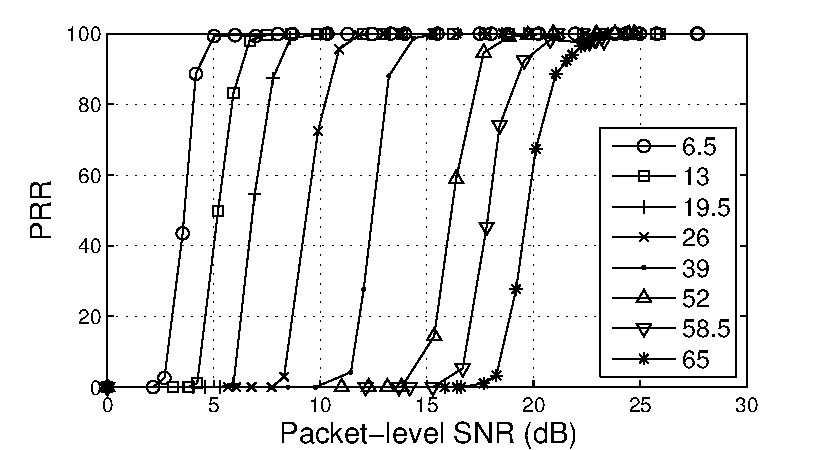
\includegraphics[width=0.4\textwidth,viewport=13 0 364 204,clip]{figures/esnr/embed_attenuator_snr_prr.pdf}
		}
\hfill%
      	\subfigure[Over real wireless channels in our testbeds, the transition region varies up to 10\dB. This loses the clear separation between rates (and so only three rates are shown for legibility).]{
			\label{fig:snr_prr_26_65}
			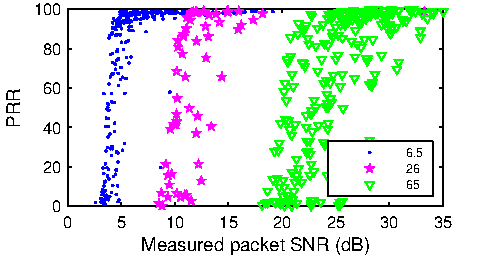
\includegraphics[width=0.4\textwidth,viewport=2 0 217 124,clip]{figures/esnr/embed_scatterplot_meas_snr_small.pdf}
		}
\hfill%
	\caption[Packet delivery over wired and real 802.11 channels.]{\label{fig:rssi_predictions}Measured (single antenna) 802.11n packet delivery over wired and real channels.}%
\end{figure}
\topheading{Packet Delivery versus RSSI/SNR\@.}
Textbook analyses of modulation schemes give delivery probability for a single signal in terms of the signal-to-noise (SNR) ratio~\cite{Goldsmith}, %The SNR is defined as the ratio of the signal power to the thermal noise power, typically expressed on a logarithmic scale in decibels, i.e., SNR = $10\log_{10}(S/N)$. 
typically expressed on a log scale in decibels.
This model holds for narrowband channels with additive white Gaussian noise. It predicts a sharp transition region of 1--2\dB over which a link changes from extremely lossy to highly reliable. This makes the SNR a valuable indicator of performance.

We generated performance curves using SNR for the \term{iwl5300} over a simple wired link with a variable attenuator and for a single transmit and receive antenna. The result is shown for all single antenna 802.11n rates in \figref{fig:snr_prr_attenuator}. 
We observe a characteristic sharp transition region for packet reception rate (PRR) versus SNR\@. This is despite the relatively wide 20\MHz channel, 56 OFDM subcarriers, coding and other bit-level operations. This is the behavior we want from a link metric in order to predict packet delivery.

In contrast, packet delivery over real wireless channels does not exhibit the same picture. \figref{fig:snr_prr_26_65} shows the measured PRR versus SNR for three sample rates (6.5, 26, and 65\Mbps) over all wireless links in our testbeds, using the same 802.11n NICs. The SNR of the transition regions can exceed 10\dB, so that some links easily work for a given SNR and others do not. There is no longer clear separation between rates. This is consistent with other reported measurements that show RSSI does not predict packet delivery for real links~\cite{aguayo_roofnet, reis_sigcomm06, snr_infocom08, zhao_sensys03}.

\begin{figure}[t]
  \centering
  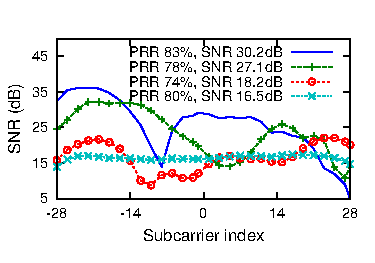
\includegraphics[width=\columnwidth,viewport=2 9 185 108,clip]{figures/esnr/embed_fsf-shape-two-links.pdf}
% viewport=2 10 170 108
  \caption{Channel gains on four links that perform about equally well at 52\Mbps. The more faded links require larger RSSIs (i.e., more transmit power) to achieve similar PRRs.}
  \label{fig:example_fsf_shape}
  % information for the links used to make above plot: 
  %srcs = [1 10 3 3];
  %dests = [9 11 2 5];
  %txpowers = [-4 20 28 20];

  % reference numbers from expt-8
  %prr = [80 83 78 74];
  %rss = [16.5 30.2 27.1 18.2];
\end{figure}

\heading{Example: RSSI vs CSI\@.}
To contrast CSI and RSSI, \figref{fig:example_fsf_shape} shows packet delivery rates, RSSIs, and subcarrier-level CSI for four links that exhibit similar performance when using the 802.11n single-stream 52\Mbps rate. Multipath causes some subcarriers to work markedly better than others although all use the same modulation and coding. These channel details, and not simply the overall signal strength as given by RSSI, affect packet delivery. The fading profiles vary significantly across the four links. One distribution is quite flat across the subcarriers, while the other three exhibit frequency-selective fading of varying degrees. Two of the links have two deeply-faded subcarriers that are more than 20\dB down from the peak.

These links harness the received power with different efficiencies.
The more faded links are more likely to have errors that must be repaired with coding, and require extra transmit power to compensate. Thus, while the performance is roughly the same, the most frequency-selective link needs a much higher overall packet SNR~(30.2\dB) than the frequency-flat link (16.5\dB). This difference of almost 14\dB highlights why RSSI-based SNR does not reliably predict performance. Fading and its effects are well-known. However, it is rare to see data that shows fading for real links and NICs because it has been difficult to measure.

\section{Effective SNR Model for 802.11n}
The example of \figref{fig:example_fsf_shape} indicated that the extra information in CSI can help explain performance for real wireless links. Here, we develop a model that can accurately predict the packet delivery probability of commodity 802.11 NICs for a given physical layer configuration operating over a given channel. We want our model to be simple and practical, so that it can be readily deployed, and to cover a wide range of physical layer configurations, so that it can be applied in many settings and for many tasks. In particular, the scope of our model is 802.11n including multiple antenna modes, including OFDM and MIMO. This scope is sufficient for many current and future networks. In our preliminary work, we have modeled delivery for single packet transmission only.

\heading{Model Design.}
The structure of our model is simple: given 1) a current CSI measurement of the RF channel between transmitter and receiver, and 2) a target physical layer configuration of the transmit and receive NICs, it predicts whether that link will reliably deliver packets in that configuration.
With this simple decision primitive, we can easily build higher layer optimization protocols. These include selecting the best rate, number of spatial streams, or transmit antenna set; whether to use 20\MHz or the entire 40\MHz channel; or choosing the lowest transmit power at which the link supports a particular rate.

For the model output, we define that the link will work, i.e., will reliably deliver packets, if we predict $\geq$90\% packet reception rate. We do not try to make predictions in the transition region during which a link changes from lossy to reliable. Predictions there are likely to be variable, and simply knowing when the link starts to work is useful information in practice.

\begin{table}
\centering
%\footnotesize
\begin{tabular}{ccc}
\toprule
Modulation & Bits/Symbol ($k$) & BER$_k$($\rho$) \\
\midrule BPSK & 1 & $Q\left(\sqrt{2\rho}\right)$ \\
QPSK & 2 & $Q\left(\sqrt{\rho}\right)$\\
QAM-16 & 4 & $\frac{3}{4}Q\left(\sqrt{\rho/5}\right)$\\
QAM-64 & 6 & $\frac{7}{12}Q\left(\sqrt{\rho/21}\right)$\\
\bottomrule
\end{tabular}
\caption{\label{tab:ber_snr}Bit error rate as a function of the symbol SNR $\rho$ for narrowband signals and OFDM modulations. $Q$ is the standard normal CDF\@.}
\end{table}


\heading{802.11 Packet Reception.}
The model must account for the action of the 802.11 receiver on the received signal. This is a complex process described in many pages of the 802.11n specification~\cite{80211n}. Our challenge is to capture it well enough with a fairly simple model. We begin by describing the main steps involved (\figref{fig:ofdm_decoding}).

First, MIMO processing separates the signals of multiple spatial streams that have been mixed by the channel. As wireless channels are frequency-selective, this operation happens separately for each subcarrier. The demodulator converts each subcarrier's symbols into the bits of each stream from constellations of several different modulations (BPSK, QPSK, QAM-16, QAM-64). This happens in much the same way as demodulating a narrowband channel. The bits are then deinterleaved to undo an encoding that spreads errors that are bursty in frequency across the data stream. A parallel to serial converter combines the bits into a single stream. Forward error correction at any of several rates (1/2, 2/3, 3/4, and 5/6) is then decoded. Finally, the descrambler exclusive-ORs the bitstream with a pseudorandom bitmask added at the transmitter to avoid data-dependent deterministic errors.

\begin{figure*}[ht!]
\centering
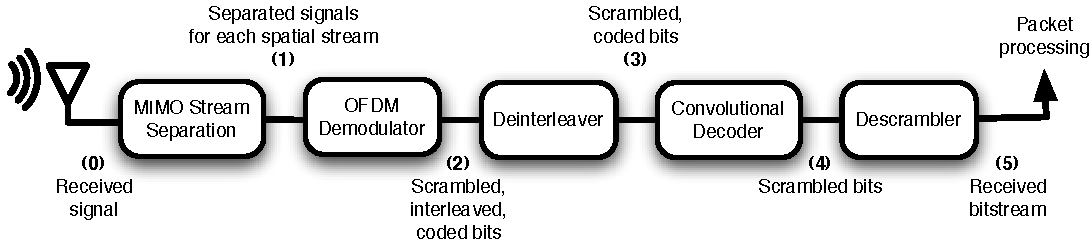
\includegraphics[width=6in]{figures/esnr/mimo_ofdm_decoding_process.pdf}
\caption[The 802.11n MIMO-OFDM decoding process.]{\label{fig:ofdm_decoding} The 802.11n MIMO-OFDM decoding process. MIMO receiver separates the RF signal~(0) for each spatial stream~(1). Demodulation converts the separated signals into bits~(2). Bits from the multiple streams are deinterleaved and combined~(3) followed by convolutional decoding~(4) to correct errors. Finally, scrambling that randomizes bit patterns is removed and the packet is processed~(5).}
\end{figure*}

\heading{Modeling Delivery.}
We build our model up from narrowband demodulation. 
Standard formulas summarized in \tabref{tab:ber_snr} relate SNR (denoted $\rho$) to bit-error rate (BER) for the modulations used in 802.11~\cite{Goldsmith}. CSI gives us the SNR values ($\rho_s$) to use for each subcarrier. For a SISO system, $\rho_s$ is given by the single entry in $H_s$.

In OFDM, decoding is applied across the demodulated bits of subcarriers. If we assume frequency-flat fading for the moment, then all the subcarriers have the same SNR\@. The link will behave the same as in our wired experiments in which RSSI reflect real performance and it will be easy to make predictions for a given SNR and modulation combination. We can use \figref{fig:snr_prr_attenuator} to measure the fixed transition points between rates and thus make our choice.

Frequency-selective fading complicates this picture as some weak subcarriers will be much more likely to have errors than others that are stronger. To model a link in this case, we turn to the notion of an \textbf{\em Effective SNR}. This is defined as the SNR that would give the \emph{same error performance on a narrowband channel}~\cite{nanda_effectiveSNR}. For example, the links in \figref{fig:example_fsf_shape} will have Effective SNR values that are nearly equal because they perform similarly, even though their RSSIs are spread over 15\dB.

The Effective SNR is \emph{not} simply the average subcarrier SNR; indeed, assuming a uniform noise floor, that average is indeed equivalent to the packet SNR derived from the RSSI\@. Instead, the Effective SNR is biased towards the weaker subcarrier SNRs because it is these subcarriers that produce most of the errors. If we ignore coding for the moment, then we can compute the Effective SNR by averaging the subcarrier BERs and then finding the corresponding SNR\@. That is:
\begin{equation}
\label{eq:effective_ber}
	\text{BER}_{\text{eff},k} = \frac{1}{52} \sum \text{BER}_k(\rho_s)
\end{equation}
\begin{equation}
\label{eq:effective_snr}
	\rho_{\text{eff},k} = \text{BER}_k^{-1}(\text{BER}_{\text{eff},k})
\end{equation}
We use $\text{BER}_k^{-1}$ to denote the inverse mapping, from BER to SNR\@. We have also called the average BER across subcarriers the effective BER, $\text{BER}_{\text{eff}}$. SoftRate estimates BER using internal receiver state~\cite{Vutukuru_SoftRate}. We compute it from channel measurements instead.

Note that the BER mapping and hence Effective SNR are functions of the modulation ($k$). That is, unlike the RSSI, a particular wireless channel will have four different Effective SNR values, one describing performance for each of the modulations. In practice, the interesting regions for the four Effective SNRs do not overlap because at a particular Effective SNR value only one modulation will be near the transition from useless (BER $\approx$0.5) to lossless (BER $\approx$0). When graphs in this paper are presented with an Effective SNR axis, we use all four values, each in the appropriate SNR range.

For 802.11n, we also model MIMO processing at the receiver. To do this we need to estimate the subcarrier SNRs for each spatial stream from the channel state matrix $H_s$. Although the standard does not specify receiver processing, 
we assume that a Minimum Mean Square Error (MMSE) receiver is used. It is computationally simple, optimal and equivalent to Maximal-Ratio Combining (MRC) for a single stream, and near optimal for multiple streams. 
All of these make it a likely choice in practice.
%This assumption allows us to use standard formulas to map channel matrices for each subcarrier (from CSI) to per-stream subcarrier SNRs.
%The $N$ per-stream MMSE output SNRs for subcarrier $s$ are 
The SNR of the $i^{\text{th}}$ stream after MMSE processing for subcarrier $s$ is 
given by $\rho_{s,i} = 1/Y_{ii}-1$, where
%\begin{equation}
%\label{eq:mmse_snr}
	$Y = \left(H_s^H H_s+I\right)^{-1}$
%\end{equation}
for $i \in [1,N]$ and $N$x$N$ identity matrix $I$~\cite{Tse}. For MIMO, the model computes the effective BER averaged across both subcarriers and streams.

Coding interacts with the notion of Effective SNR in a way that is difficult to analyze. One challenge is that the ability to correct bit errors depends on the position of the errors in the data stream. To sidestep this problem, we rely on the interleaving that randomizes the coded bits across subcarriers and spatial streams. Assuming perfect interleaving and robust coding, bit errors in the stream should look no different from bit errors for flat channels (but at a lower SNR). Thus our estimate of the effective BER in \eqref{eq:effective_ber} will accurately reflect the uncoded error performance of the link. Our algorithm now proceeds as in the case of a flat-fading channel described above: we take the computed Effective SNR value and use the measurements from a flat-fading link (\figref{fig:snr_prr_attenuator}) to determine transmission success or failure. As in CHARM~\cite{Judd_CHARM}, we support different packet lengths with different SNR thresholds.

Note that this procedure differs from the typical approach of simulation-based analyses~\cite{Kant_fla, Liu_EESM, Nortel_3g}, that instead map the \emph{uncoded} BER estimate such as we compute to a \emph{coded} BER estimate by means of a simple log-linear approximation. They then use the coded BER estimate, and the length of the target transmission, to directly compute the packet delivery rate of the link. We believe our method of thresholding the Effective SNR is better because it directly accommodates variation in the receiver implementation. Different devices may have different \emph{noise figures}, a measure of how much signal strength is lost in the internal RF circuitry of the NIC\@. They may implement soft Viterbi decoders with more or fewer soft bits for their internal state, or indeed might do hard decoding instead. A receiver could use the optimal Maximum Likelihood MIMO decoder that has exponential complexity for small constellations like BPSK, but revert to the imperfect but more efficient MMSE at higher modulations. All of these can be easily expressed, albeit maybe approximately, as (perhaps modulation-dependent) shifts in the Effective SNR thresholds. In contrast, changing these parameters in the simulation approach involves changing the internals of the calculation.

\heading{Protocol Details.} Effective SNR calculations can be performed by either receiver or transmitter, and each has advantages. For it to make decisions, the transmitter must know the receiver's thresholds for the different rates; these are fixed for a particular model of NIC and can be shared once, e.g., during association. The transmitter also needs up-to-date CSI: either from feedback or estimated from the reverse path. Alternately, the receiver can request rates and select antennas directly using the new Link Adaptation Control field of any 802.11n QoS packet~\cite[\S7.1.3.5a]{80211n}. This obviates sending CSI, but the calculation instead requires that the transmitter share its spatial mappings, i.e. how it maps spatial streams to transmit antennas. These are likely to change less frequently than the channel, if at all. Finally, when operating in either mode with fewer transmit streams than antennas, the transmitter must occasionally send a short probe packet with all antennas to measure the full CSI\@.

\heading{Summary and Example.} Combining the above steps, our model consists of the following: 1) CSI is obtained and a test configuration is chosen; 2) the MMSE expression is used to compute per-stream, subcarrier SNRs from the CSI for the test number of streams; 3) the Effective SNR is computed from the per-stream, subcarrier SNRs for the test modulation; and 4) the Effective SNR is compared against the pre-determined threshold for the test modulation and coding to predict whether the link will deliver packets.

\begin{figure}[t]
  \centering
  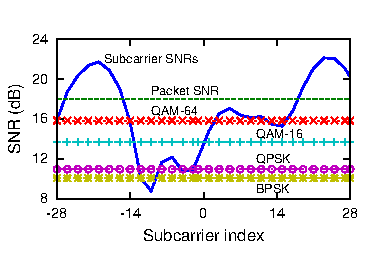
\includegraphics[width=0.9\columnwidth,viewport=0 9 180 111,clip]{figures/esnr/embed_fsf-shape-eff-snr-s3d5-txpower-20.pdf}
  % viewport=0 7 173 113
  \vspace{-4pt}
  \caption{Sample faded link showing the packet SNR and Effective SNRs for different modulations. BPSK has the lowest Effective SNR, but it needs less energy to decode.}
  \label{fig:eff_example}
  \vspace{-3pt}
\end{figure}


As an example, \figref{fig:eff_example} shows the CSI for a SISO link (steps 1--2) as a fading profile across subcarriers, with the computed Effective SNRs for all modulations (step 3). These Effective SNRs are compared with pre-determined thresholds (\figref{fig:snr_prr_attenuator}) to correctly predict that the best working rate will be 39\Mbps. 
Note that these Effective SNRs are well below the RSSI-based packet SNR that is biased towards the stronger subcarriers (note the logarithmic $y$-axis scale). This link does a poor job of harnessing the received power because it is badly faded, so its SNR is a poor predictor of rate.

\chapter{Application/Evaluation of Effective SNR}
\label{chap:esnr_eval}
\chapter{Wireless for Datacenters}
\label{chap:flyways_intro}
\chapter{Evaluation of 60\GHz Flyways}
\label{sec:datacenter_eval}
\chapter{Discussion}
\label{chap:discussion}
\ifx\mainfile\undefined
%  ========================================================================
%  Copyright (c) 2006-2011 The University of Washington
%
%  Licensed under the Apache License, Version 2.0 (the "License");
%  you may not use this file except in compliance with the License.
%  You may obtain a copy of the License at
%
%      http://www.apache.org/licenses/LICENSE-2.0
%
%  Unless required by applicable law or agreed to in writing, software
%  distributed under the License is distributed on an "AS IS" BASIS,
%  WITHOUT WARRANTIES OR CONDITIONS OF ANY KIND, either express or implied.
%  See the License for the specific language governing permissions and
%  limitations under the License.
%  ========================================================================
%
 
\documentclass [11pt, twoside] {uwthesis}

\usepackage{color}
\usepackage{url}
\usepackage{amsmath}
\usepackage{amsfonts}
\usepackage[bookmarks,
	hidelinks,
	plainpages=false,
	pdfpagelabels,
	pagebackref=true,
            ]{hyperref}
\renewcommand*{\backref}[1]{}% for backref < 1.33 necessary
\renewcommand*{\backrefalt}[4]{%
  \ifcase #1 %
    (No citations.)%
  \or
    (Cited on page #2.)%
  \else
    (Cited on pages #2.)%
  \fi
}

\newcommand{\biburl}[1]{{\tt<}\url{#1}{\tt>}}

\hypersetup{%
pdfauthor = {Daniel Chaim Halperin},
pdftitle = {Simplifying the Configuration of 802.11 Wireless Networks with Effective SNR},
pdfsubject = {Ph.D. Dissertation},
pdfkeywords = {},
pdfcreator = {University of Washington, Computer Science and Engineering},
pdfproducer = {},
bookmarksopen = {true},
pdfpagelayout = {TwoColumnRight},
}

\usepackage{footnotebackref}
%%%%%%%%%%%%%%%%%%%%%%%%%%%%%%%%%%%%%%%%%%%%%%%%%%%%%%
%%%        Formatting sections                     %%%
%%%%%%%%%%%%%%%%%%%%%%%%%%%%%%%%%%%%%%%%%%%%%%%%%%%%%%
\newcommand{\algref}[1]{Algorithm~\ref{#1}}
\newcommand{\chapref}[1]{Chapter~\ref{#1}}
\renewcommand{\eqref}[1]{Equation~\ref{#1}}
\newcommand{\figref}[1]{Figure~\ref{#1}}
\newcommand{\secref}[1]{\S\ref{#1}}
\newcommand{\tabref}[1]{Table~\ref{#1}}
\newcommand{\heading}[1]{\vspace{4pt}\noindent\textbf{#1}}
\newcommand{\topheading}[1]{\noindent\textbf{#1}}
\newcommand{\noheading}[0]{\vspace{4pt}\noindent}

%%%%%%%%%%%%%%%%%%%%%%%%%%%%%%%%%%%%%%%%%%%%%%%%%%%%%%
%%%        XXX and other warnings                  %%%
%%%%%%%%%%%%%%%%%%%%%%%%%%%%%%%%%%%%%%%%%%%%%%%%%%%%%%
\newcommand{\xxx}[1]{\textit{\color{red}XXX #1}}

%%%%%%%%%%%%%%%%%%%%%%%%%%%%%%%%%%%%%%%%%%%%%%%%%%%%%%
%%%        Units                                   %%%
%%%%%%%%%%%%%%%%%%%%%%%%%%%%%%%%%%%%%%%%%%%%%%%%%%%%%%
\usepackage{xspace}
\newcommand{\unitsep}{\texorpdfstring{\,}{ }}
\def\unit#1{% from: http://www.tex.ac.uk/cgi-bin/texfaq2html?label=csname "Defining a macro from an argument"
  \expandafter\def\csname #1\endcsname{\unitsep\text{#1}\xspace}%
}
\def\varunit#1#2{% from: http://www.tex.ac.uk/cgi-bin/texfaq2html?label=csname "Defining a macro from an argument"
  \expandafter\def\csname #1\endcsname{\unitsep\text{#2}\xspace}%
}
\unit{GHz}
\unit{MHz}
\unit{kHz}
\unit{Gbps}
\unit{Mbps}
\unit{KB}
\unit{dB}
\unit{dBi}
\unit{dBm}
\unit{W}
\unit{mW}
\varunit{uW}{$\mu$W}
\unit{ms}
\varunit{us}{$\mu$s}
\unit{h}
\unit{m}
\unit{s}
\unit{km}
\unit{cm}
\unit{mm}
\varunit{mmsq}{mm$^\text{2}$}
\varunit{insq}{in$^\text{2}$}
\newcommand{\degree}{\ensuremath{^\circ}\xspace}
\newcommand{\degrees}{\degree}
%%%%%%%%%%%%%%%%%%%%%%%%%%%%%%%%%%%%%%%%%%%%%%%%%%%%%%%%%%%%%%%%%%%%%%%%%%%%%%%%%%%%%%
% Euler for math | Palatino for rm | Helvetica for ss | Courier for tt
%
% From: http://www.tug.org/mactex/fonts/LaTeX_Preamble-Font_Choices.html
%%%%%%%%%%%%%%%%%%%%%%%%%%%%%%%%%%%%%%%%%%%%%%%%%%%%%%%%%%%%%%%%%%%%%%%%%%%%%%%%%%%%%%
\renewcommand{\rmdefault}{ppl} % rm
\usepackage[scaled]{helvet} % ss
\usepackage{courier} % tt
\usepackage{eulervm} % a better implementation of the euler package (not in gwTeX)
\normalfont
\usepackage[T1]{fontenc}
%%%%%%%%%%%%%%%%%%%%%%%%%%%%%%%%%%%%%%%%%%%%%%%%%%%%%%%%%%%%%%%%%%%%%%%%%%%%%%%%%%%%%%

%%%%%%%%%%%%%%%%%%%%%%%%%%%%%%%%%%%%%%%%%%%%%%%%%%%%%%
%%%        Figures                                 %%%
%%%%%%%%%%%%%%%%%%%%%%%%%%%%%%%%%%%%%%%%%%%%%%%%%%%%%%
\usepackage{graphicx}
% Caption package both lets you set the spacing between figure and caption
% and also makes the \figref{} point to the right place.
\usepackage[font=bf,aboveskip=6pt,belowskip=-4mm]{caption}
% Allow subfigures, make them bold
\usepackage[bf,BF,small]{subfigure}
% List of figures
\setcounter{lofdepth}{2}  % Print the chapter and sections to the lot

%%%%%%%%%%%%%%%%%%%%%%%%%%%%%%%%%%%%%%%%%%%%%%%%%%%%%%
%%%        Lists with reduced spacing              %%%
%%%%%%%%%%%%%%%%%%%%%%%%%%%%%%%%%%%%%%%%%%%%%%%%%%%%%%
\usepackage{enumitem}

%%%%%%%%%%%%%%%%%%%%%%%%%%%%%%%%%%%%%%%%%%%%%%%%%%%%%%
%%%        Fancy tables                            %%%
%%%%%%%%%%%%%%%%%%%%%%%%%%%%%%%%%%%%%%%%%%%%%%%%%%%%%%
\usepackage{tabulary}
\usepackage{booktabs}

%%%%%%%%%%%%%%%%%%%%%%%%%%%%%%%%%%%%%%%%%%%%%%%%%%%%%%
%%%        Formatting techniques/tools/etc.        %%%
%%%%%%%%%%%%%%%%%%%%%%%%%%%%%%%%%%%%%%%%%%%%%%%%%%%%%%
\newcommand{\term}[1]{\texttt{#1}}

\begin{document}
 
\textpages
\setcounter{chapter}{7} % Set to n-1!
\fi
%%%%%%%%%%%%%%%%%%%%%%%%%%%%%%%%%%

\cleardoublepage
\chapter{Future Work}
\label{chap:future}

%%%%%%%%%%%%%%%%%%%%%%%%%%%%%%%%%%
\ifx\mainfile\undefined
%
% ==========   Bibliography   ==========
%
%\nocite{*}   % include everything in the uwthesis.bib file
\bibliographystyle{plain}
\bibliography{dhalperi_thesis}

\end{document}
\fi

\ifx\mainfile\undefined
%  ========================================================================
%  Copyright (c) 2006-2011 The University of Washington
%
%  Licensed under the Apache License, Version 2.0 (the "License");
%  you may not use this file except in compliance with the License.
%  You may obtain a copy of the License at
%
%      http://www.apache.org/licenses/LICENSE-2.0
%
%  Unless required by applicable law or agreed to in writing, software
%  distributed under the License is distributed on an "AS IS" BASIS,
%  WITHOUT WARRANTIES OR CONDITIONS OF ANY KIND, either express or implied.
%  See the License for the specific language governing permissions and
%  limitations under the License.
%  ========================================================================
%
 
\documentclass [11pt, twoside] {uwthesis}

\usepackage{color}
\usepackage{url}
\usepackage{amsmath}
\usepackage{amsfonts}
\usepackage[bookmarks,
	hidelinks,
	plainpages=false,
	pdfpagelabels,
	pagebackref=true,
            ]{hyperref}
\renewcommand*{\backref}[1]{}% for backref < 1.33 necessary
\renewcommand*{\backrefalt}[4]{%
  \ifcase #1 %
    (No citations.)%
  \or
    (Cited on page #2.)%
  \else
    (Cited on pages #2.)%
  \fi
}

\newcommand{\biburl}[1]{{\tt<}\url{#1}{\tt>}}

\hypersetup{%
pdfauthor = {Daniel Chaim Halperin},
pdftitle = {Simplifying the Configuration of 802.11 Wireless Networks with Effective SNR},
pdfsubject = {Ph.D. Dissertation},
pdfkeywords = {},
pdfcreator = {University of Washington, Computer Science and Engineering},
pdfproducer = {},
bookmarksopen = {true},
pdfpagelayout = {TwoColumnRight},
}

\usepackage{footnotebackref}
%%%%%%%%%%%%%%%%%%%%%%%%%%%%%%%%%%%%%%%%%%%%%%%%%%%%%%
%%%        Formatting sections                     %%%
%%%%%%%%%%%%%%%%%%%%%%%%%%%%%%%%%%%%%%%%%%%%%%%%%%%%%%
\newcommand{\algref}[1]{Algorithm~\ref{#1}}
\newcommand{\chapref}[1]{Chapter~\ref{#1}}
\renewcommand{\eqref}[1]{Equation~\ref{#1}}
\newcommand{\figref}[1]{Figure~\ref{#1}}
\newcommand{\secref}[1]{\S\ref{#1}}
\newcommand{\tabref}[1]{Table~\ref{#1}}
\newcommand{\heading}[1]{\vspace{4pt}\noindent\textbf{#1}}
\newcommand{\topheading}[1]{\noindent\textbf{#1}}
\newcommand{\noheading}[0]{\vspace{4pt}\noindent}

%%%%%%%%%%%%%%%%%%%%%%%%%%%%%%%%%%%%%%%%%%%%%%%%%%%%%%
%%%        XXX and other warnings                  %%%
%%%%%%%%%%%%%%%%%%%%%%%%%%%%%%%%%%%%%%%%%%%%%%%%%%%%%%
\newcommand{\xxx}[1]{\textit{\color{red}XXX #1}}

%%%%%%%%%%%%%%%%%%%%%%%%%%%%%%%%%%%%%%%%%%%%%%%%%%%%%%
%%%        Units                                   %%%
%%%%%%%%%%%%%%%%%%%%%%%%%%%%%%%%%%%%%%%%%%%%%%%%%%%%%%
\usepackage{xspace}
\newcommand{\unitsep}{\texorpdfstring{\,}{ }}
\def\unit#1{% from: http://www.tex.ac.uk/cgi-bin/texfaq2html?label=csname "Defining a macro from an argument"
  \expandafter\def\csname #1\endcsname{\unitsep\text{#1}\xspace}%
}
\def\varunit#1#2{% from: http://www.tex.ac.uk/cgi-bin/texfaq2html?label=csname "Defining a macro from an argument"
  \expandafter\def\csname #1\endcsname{\unitsep\text{#2}\xspace}%
}
\unit{GHz}
\unit{MHz}
\unit{kHz}
\unit{Gbps}
\unit{Mbps}
\unit{KB}
\unit{dB}
\unit{dBi}
\unit{dBm}
\unit{W}
\unit{mW}
\varunit{uW}{$\mu$W}
\unit{ms}
\varunit{us}{$\mu$s}
\unit{h}
\unit{m}
\unit{s}
\unit{km}
\unit{cm}
\unit{mm}
\varunit{mmsq}{mm$^\text{2}$}
\varunit{insq}{in$^\text{2}$}
\newcommand{\degree}{\ensuremath{^\circ}\xspace}
\newcommand{\degrees}{\degree}
%%%%%%%%%%%%%%%%%%%%%%%%%%%%%%%%%%%%%%%%%%%%%%%%%%%%%%%%%%%%%%%%%%%%%%%%%%%%%%%%%%%%%%
% Euler for math | Palatino for rm | Helvetica for ss | Courier for tt
%
% From: http://www.tug.org/mactex/fonts/LaTeX_Preamble-Font_Choices.html
%%%%%%%%%%%%%%%%%%%%%%%%%%%%%%%%%%%%%%%%%%%%%%%%%%%%%%%%%%%%%%%%%%%%%%%%%%%%%%%%%%%%%%
\renewcommand{\rmdefault}{ppl} % rm
\usepackage[scaled]{helvet} % ss
\usepackage{courier} % tt
\usepackage{eulervm} % a better implementation of the euler package (not in gwTeX)
\normalfont
\usepackage[T1]{fontenc}
%%%%%%%%%%%%%%%%%%%%%%%%%%%%%%%%%%%%%%%%%%%%%%%%%%%%%%%%%%%%%%%%%%%%%%%%%%%%%%%%%%%%%%

%%%%%%%%%%%%%%%%%%%%%%%%%%%%%%%%%%%%%%%%%%%%%%%%%%%%%%
%%%        Figures                                 %%%
%%%%%%%%%%%%%%%%%%%%%%%%%%%%%%%%%%%%%%%%%%%%%%%%%%%%%%
\usepackage{graphicx}
% Caption package both lets you set the spacing between figure and caption
% and also makes the \figref{} point to the right place.
\usepackage[font=bf,aboveskip=6pt,belowskip=-4mm]{caption}
% Allow subfigures, make them bold
\usepackage[bf,BF,small]{subfigure}
% List of figures
\setcounter{lofdepth}{2}  % Print the chapter and sections to the lot

%%%%%%%%%%%%%%%%%%%%%%%%%%%%%%%%%%%%%%%%%%%%%%%%%%%%%%
%%%        Lists with reduced spacing              %%%
%%%%%%%%%%%%%%%%%%%%%%%%%%%%%%%%%%%%%%%%%%%%%%%%%%%%%%
\usepackage{enumitem}

%%%%%%%%%%%%%%%%%%%%%%%%%%%%%%%%%%%%%%%%%%%%%%%%%%%%%%
%%%        Fancy tables                            %%%
%%%%%%%%%%%%%%%%%%%%%%%%%%%%%%%%%%%%%%%%%%%%%%%%%%%%%%
\usepackage{tabulary}
\usepackage{booktabs}

%%%%%%%%%%%%%%%%%%%%%%%%%%%%%%%%%%%%%%%%%%%%%%%%%%%%%%
%%%        Formatting techniques/tools/etc.        %%%
%%%%%%%%%%%%%%%%%%%%%%%%%%%%%%%%%%%%%%%%%%%%%%%%%%%%%%
\newcommand{\term}[1]{\texttt{#1}}

\begin{document}
 
\textpages
\setcounter{chapter}{9} % Set to n-1!
\fi
%%%%%%%%%%%%%%%%%%%%%%%%%%%%%%%%%%

\cleardoublepage
\chapter{Conclusions and Future Work}
\label{chap:conclusion}

Modern wireless devices can provide flexible, portable, high-performance connectivity at low cost. This unprecedented functionality is poised to enable a new class of rich applications built by combining functionality from many devices. The key missing component is a network connectivity layer that ``just works'', providing good performance overall and quickly adapting to changing application demands and mobile wireless environments.

There are two components to such a network layer. The first is a protocol to connect the devices logically. For the example context of 802.11n, this is readily available in the form of Wi-Fi Direct~\cite{wifi_direct}, a recently standardized specification for building wireless peer-to-peer networks targeted at these applications. Support for Wi-Fi Direct is actively being developed in major consumer operating systems including Linux, Mac OS X, Windows, and Android.

The focus of my thesis is on the second key component: A way to configure the physical layer parameters and network topology to best meet application needs. The nature of modern wireless technology and heterogeneity of wireless devices combined with the inherent multi-device coordination problems that applications necessitate leads to large configuration state spaces from which the network must find a good operating point. In this thesis, I have demonstrated that my Effective SNR model provides a practical mechanism to cut through these large spaces and efficiently configure the physical layer. I have also shown that it can flexibly handle a wide variety of applications and parameters that no prior approaches considered in tandem.

In this chapter I summarize my thesis and its contributions and present next steps for this work.

\section{Thesis and Contributions}
My thesis is that \emph{it is possible to rapidly and accurately predict how well different configurations of MIMO and OFDM wireless links will perform in practice, using a small set of wireless channel measurements}. I demonstrated this thesis by building an Effective SNR-based model for wireless networks and evaluating it in the context of IEEE 802.11n.

My Effective SNR model unifies wireless network configuration using a simple interface, taking as input a MIMO and OFDM channel measurement and transmitter and receiver device configurations, and producing a single output bit that predicts whether that combination will deliver packets. This flexible API can express a wide class of applications, as illustrated by the algorithms I presented in \chapref{chap:delivery}, \chapref{chap:rate}, and \chapref{chap:applications}.

I demonstrated that this model is practical because it has low overhead and can be deployed using commodity wireless hardware today. My model uses measurements already taken by devices in order to receive packets, and can compute its output in much less time than it takes to transmit a packet. In most cases, only a few bytes that represent application decisions need to be exchanged, such as a receiver feeding back a particular requested rate to a transmitter. And my detailed prototype evaluation of the model in a wide variety of applications provides experimental proof that this model is practical and accurate for real devices operating in real wireless channels. I used this prototype to apply model to a wide range of applications, and showed that it has good performance that extends to large search spaces and fast mobile channels.

My specific contributions are as follows.

\begin{itemize}[leftmargin=0.5cm,parsep=1ex,itemsep=1ex,topsep=1ex]
\item First, I developed a model to predict the error performance of different transmitter and receiver configurations on real MIMO-OFDM wireless channels. This model is flexible to support a wide variety of transmitter and receiver device capabilities and applications, and includes considerations of practical factors such as measurement errors, different device implementations, and practical protocols. I also detailed how to use this model in a system that can solve a large number and variety of configuration problems.
\item Second, I presented an implementation of this system in the context of 802.11n using a commodity commercial wireless device. This prototype demonstrated my model's feasibility in practice and handles the practical considerations of operation over real links using real, non-ideal hardware. This includes a detailed experimental evaluation of my system that shows that this model accurately predicts packet delivery over real 802.11n wireless links in practice.
\item Third, I evaluated this system in the context of a wide variety of 802.11n applications, and quantified the application performance gains when using my Effective SNR metric over versions that use the Packet SNR based on RSSI measurements available today.
\item Finally, as part of my thesis I have produced an 802.11n research platform based on open-source Linux kernel drivers, open-source application code, and commodity Intel 802.11n devices using closed-source firmware that I customized.
%that uses commodity 802.11n wireless devices to measure the 802.11n CSI for the wireless channel, and use this tool to apply my model to real measured 802.11n channels.
I have released this tool publicly, and at the time of writing it is in use at 23 universities, research labs, and corporations.
\end{itemize}

\section{Future Work}
In this section, I consider paths for future research.

\subsection{Practical Benefits of Beamforming}
Transmit beamforming is a well-studied area of research in communications theory. Most theoretical systems aim to optimize Shannon capacity using ideal hardware, in which case the well known water-filling approach~\cite[p. 183]{Tse} optimizes performance by allocating power across subchannels proportional to SNR, using the singular value decomposition. This approach may be inefficient in practice for two reasons. First, real transmit hardware can only support signals with a particular dynamic range, and so cannot perfectly support water-filling. Secondly, in practical systems like 802.11, different subchannels are modulated identically and thus cannot make good use of the asymmetric power across subchannels. Instead, the Effective SNR model can be used to evaluate allocations of power with the goal of minimizing bit errors and finding the best working modulation and coding scheme across all subchannels.

\subsection{Spatial Reuse}
Another area of further research is understanding and managing spatial reuse, that is, understanding when multiple transmitters can send concurrently on the same frequency band. This problem is the subject of great importance in today's AP wireless networks, but will likely be ameliorated to a large extent in future wireless networks that can take advantage of multiple channels. Still, existing work has shown large gains from spatial reuse especially in the area of eliminating corner cases of hidden terminals that can degrade link performance to almost nothing. Today's solutions such as CSMA/CA use expensive distributed coordination mechanisms (i.e., RTS/CTS~\cite{Karn_MACA}) with large overheads that are often disabled in practice, and today's research proposals on spatial reuse for Wi-Fi~\cite{Shrivastava_CENTAUR,Vutukuru_CMAP} have simply fixed the entire network to a single rate during experiments because of the large search space. Communications theory has also defined an Effective SINR notion that takes interference into account; extending my model to support a practical version of this notion would likely be useful as well.

\subsection{Saving Energy with Effective SNR}
Effective SNR could be highly integrated into the development of better methods to manage the power consumption of battery-operated devices. In particular, clients could select access points or relays with the express aim of minimizing wake time. By choosing a close relay that uses fast rates, a client can spend less time awake. By disabling receive antennas on the mobile device and using advanced mechanisms such as beamforming on the transmitter, the client can make further power savings. I highlighted the importance of these 802.11n parameters in an earlier measurement study~\cite{Halperin_Power}, but have not performed follow-up research.

\subsection{Integration into Wi-Fi Direct}
Finally, I would like to integrate my thesis into a modern flexible networking system to really build a flexible application layer that ``just works''. The immediately available practical environment is that of Wi-Fi Direct, which is close to being refined enough to support experiments. Though my thesis has demonstrated the practical benefits of my model and its deployment in a variety of individual applications, building a working combined system would provide invaluable practical experience and research lessons.

\section{Summary}
The way that chaotic wireless systems such as 802.11 are configured today relies on probing, for rate adaptation and for a host of other applications. This probing is the standard strategy because communications-theoretic approaches to configuring network parameters are considered too inaccurate to work well. However, in my thesis I have shown the opposite, namely that it is indeed possible to connect theory back to real wireless systems operating in real wireless channels. I have presented an Effective SNR model for wireless systems that use modern physical layer techniques like MIMO and OFDM, and shown that it works well for real wireless devices operating in real wireless channels for the state-of-the-art wireless system in use today, IEEE 802.11n. Going forward, I hope that Effective SNR will be integrated into the control plane for the dense future wireless networks and help enable the next generation of device-to-device wireless applications.

%%%%%%%%%%%%%%%%%%%%%%%%%%%%%%%%%%
\ifx\mainfile\undefined
%
% ==========   Bibliography   ==========
%
%\nocite{*}   % include everything in the uwthesis.bib file
\bibliographystyle{plain}
\bibliography{dhalperi_thesis}

\end{document}
\fi


 

% ==========   End notes   ==========

\printendnotes

%
% ==========   Bibliography   ==========
%
%\nocite{*}   % include everything in the uwthesis.bib file
\bibliographystyle{plain}
\bibliography{dhalperi_thesis}
%
% ==========   Appendices
%
\appendix
\raggedbottom\sloppy
%
% ==========   Vita   ==========
%
\vita{Jim Fox is a Senior Software Engineer at the University of Washington.
His duties do not include maintaining this package.  It is rather
an avocation which he maintains as he deems fit.

He welcomes your comments to {\tt fox@washington.edu}.
}

\end{document}
